% HEXIS NeurIPS 2026 Submission — Main Document v2
\documentclass[10pt]{article}
\usepackage{neurips_2026}

% Packages
\usepackage[utf8]{inputenc}
\usepackage[T1]{fontenc}
\usepackage{amsmath,amssymb,amsfonts}
\usepackage{graphicx}
\graphicspath{{/home/dgonier/experiments/figures/}{../../figures/}{../figures/}{../}}
\usepackage{booktabs}
\usepackage{hyperref}
\usepackage{natbib}
\usepackage{xcolor}
\usepackage{subcaption}
\usepackage{microtype}
\usepackage{multirow}
\usepackage{pifont}
\usepackage{enumitem}
\usepackage{bm}
\newcommand{\cmark}{\ding{51}}
\newcommand{\xmark}{\ding{55}}

\title{HEXIS: Compiled Dispositional Memory Through Enmeshed Networks}

% NeurIPS: double-blind — no author info at submission
\author{Anonymous}
\date{}

\begin{document}
\maketitle

% Three single-paragraph variations follow (NeurIPS abstract = one paragraph).
% V_NARRATIVE is currently active. Swap by uncommenting a different
% \begin{abstract}...\end{abstract} block.
%
% All versions follow user style rules: no em dashes, no negative parallelism
% ("not X but Y"), no AI vocabulary tells (delve, realm, landscape, tapestry,
% pivotal, transformative, etc.), no chatbot closers. See ~/.claude/AI_TELLS.md.

% =====================================================================
% V_NARRATIVE (~245 words) — ACTIVE.
% Single paragraph, narrative flow, headline numbers only.
% =====================================================================
\begin{abstract}
We introduce \textbf{enmeshed networks}, a parameter-efficient architectural pattern in which a lightweight module shares the forward pass of a frozen host model, reading and writing hidden states at every layer while remaining cleanly removable. Existing approaches to persistent memory and persistent conditioning face a fundamental trade-off: context-window methods (RAG, system prompts, MemGPT) consume tokens and are vulnerable to adversarial override, while parameter methods (LoRA, adapters) require per-domain gradient updates and lose effect on out-of-distribution tasks. An enmeshed network addresses this trade-off by asynchronously compiling a private secondary context—disposition, memory, and domain knowledge—through the frozen host into per-layer low-rank modulation tensors that condition subsequent primary-context forward passes without consuming context tokens or requiring gradient updates. We instantiate this pattern as \textbf{HEXIS}, which modulates a frozen transformer's Q and V projections using tensors compiled from a persistent knowledge graph; the graph updates from session-level reflection and recompiles into new modulation tensors via a single forward pass (${\sim}20$\,s), enabling experience-adaptive behaviour without gradient updates. We evaluate on two axes: \textit{Stance Retention} --- across five escalating levels of adversarial pressure on Qwen3.5-4B-Instruct, in-context belief conditioning capitulates at or below level~3 (0\% conviction held at $\geq$4), whereas HEXIS maintains stated beliefs 83\% of the time---and \textit{agentic capability}---on $\tau^3$-bench (4 domains, 3-judge audit), HEXIS raises the audited pass rate by $+10$\,pp (paired McNemar $p{=}0.043$), with $+24$\,pp on the held-out banking domain ($p{=}0.016$ on the full panel), where a compute-matched LoRA baseline lifts only $+8$\,pp. The mechanism scales and transfers across model families on the dispositional and teacher-loop sub-mechanisms: Qwen3.6-27B reproduces the dispositional lift at $+24$\,pp stance retention ($n{=}240$), Mistral-Ministral-8B's full-collapse rate drops from 40\% to 25\% under adversarial pressure ($n{=}240$), and a controlled hint-injection experiment on Mistral airline flips a previously-zero failure mode from 0/5 to 3/4 audited pass while a non-hint-receiving baseline holds at 0/5. The $d^*$ direction-injection sub-mechanism does not transfer to Mistral airline at the scales we tested ($n{=}60$ scale-sweep, audited).
\end{abstract}

% =====================================================================
% V_HEADLINE (~210 words) — Tighter, more numbers-forward.
% Trades the "memory-is-either-X-or-Y" framing for a faster jump to results.
% =====================================================================
% \begin{abstract}
%
% We introduce \textbf{enmeshed networks}, a parameter-efficient architectural primitive in which a lightweight module shares the forward pass of a frozen host, reading and writing hidden states at every layer while remaining cleanly removable. An enmeshed network processes a private parallel context: a structured subcontext compiled into per-layer modulation tensors that shape the primary context's computation at zero token cost, without competing for attention against the conversation it is meant to support. We instantiate this primitive as \textbf{HEXIS}, compiled stance memory for frozen transformers via low-rank Q/V modulation, with a structured memory schema (the Mind Tree) compiled into persistent modulation tensors. Three findings on Qwen3.5-4B: in-context belief conditions capitulate to a flat 3.0/5 conviction (0\% $\geq$4-conviction hold) under five escalating levels of illegitimate adversarial pressure, while HEXIS holds 83\%; on $\tau^3$-bench (4 domains, 3-judge audited) HEXIS lifts pass rate by $+10$pp ($p=0.043$) with $+24$pp on the held-out banking domain that a compute-matched LoRA control only lifts by $+8$pp; and calibrated HEXIS+LoRA composition (decode-only $d^*$ injection, $d^*$ re-extracted on the LoRA-merged model) reaches $63\%$ audited overall, $+5$pp over HEXIS-alone and $+10$pp over LoRA-only. Code anonymised for review.
%
% \end{abstract}

% =====================================================================
% V_PUNCHY (~155 words) — Most compressed.
% One architectural sentence, three result sentences, close. Use if page
% pressure is severe.
% =====================================================================
% \begin{abstract}
%
% We introduce \textbf{enmeshed networks}, a lightweight parametric module that shares the forward pass of a frozen host, reading and writing hidden states at every layer while remaining cleanly removable. We instantiate this primitive as \textbf{HEXIS}: compiled stance memory for frozen transformers via low-rank Q/V modulation, with a structured memory schema (the Mind Tree) compiled into persistent modulation tensors. Across five escalating levels of illegitimate adversarial pressure on Qwen3.5-4B, in-context conditions capitulate to flat 3.0/5 conviction (0\% $\geq$4-conviction hold) while HEXIS holds 83\%. On $\tau^3$-bench (3-judge audited), HEXIS lifts pass rate by $+10$pp ($p=0.043$), with $+24$pp on the held-out banking domain that a compute-matched LoRA control only lifts $+8$pp. Calibrated HEXIS+LoRA composition reaches $63\%$ audited overall, beating either alone. Code anonymised for review.
%
% \end{abstract}

\section{Introduction}

The dominant paradigm for equipping large language models with memory places memory as \emph{content} in a single shared context window. RAG retrieves documents into the prompt. MemGPT manages a working-memory buffer of text. Reflexion accumulates verbal reflections as prompt prefixes. System prompts define behaviour through instructions the model reads. Methods that encode information into parameters---LoRA adapters, learned soft prompts---avoid the context window but require gradient descent per adaptation and produce fixed representations that do not update from ongoing experience. In all cases, the model's memory is either explicit content competing for attention in a single context, or frozen parameters set at training time. We are missing a third option: a \emph{non-context-mediated memory channel} that persists across forward passes, adapts from experience without weight updates, and operates outside the chain-of-thought an adversary can argue within. By analogy to dual-process accounts of human memory \citep{graf1985implicit, schacter1987implicit} --- the butcher whose perceptual priors have been reshaped by decades of experience does not consult a lookup table; his eyes simply land on different features --- we want an architectural channel that shapes \emph{how} the model processes its input rather than \emph{what} it reads. We make this analogy as motivation, not as a strict mechanistic claim (\S\ref{sec:related_work}).

The current architecture forces all memory into a single inspectable channel, with three well-known failure modes. First, \emph{dilution}: as the context window fills with conversation, task content, or adversarial filler, the memory competes for attention with everything else and its influence degrades. Second, \emph{sycophancy}: the model can inspect its own memory, and an adversarial interlocutor can argue against the stated beliefs until the model abandons them. Third, \emph{cost}: every token of memory is a token of context, incurring linear attention cost at every generation step. These failures manifest across application domains: user preference tracking that dilutes over multi-turn conversation, research agents whose convictions fold under peer pressure, agentic strategy logs that crowd out task context, and codebase knowledge that scales linearly with repository size.

We address all three failure modes by introducing a new architectural primitive---the \emph{enmeshed network}---and instantiating it as HEXIS (Hidden Enmeshed eXperiential Identity States; the name is a label, the technical claim is operational), a system that implements compiled stance memory for frozen transformers. Where existing approaches force all memory into a single context window where it competes for attention, HEXIS opens a \emph{parallel context channel}: a structured cognitive schema (the Mind Tree) is processed through the same host model in a private forward pass and compiled into low-rank modulation tensors that merge with the primary context's computation. The primary context carries the conversation. The parallel context carries the disposition. The two share the same forward pass---the enmeshed network reads the host's hidden states and writes modulations at each patched layer---but the parallel context never occupies primary context positions and never competes for the primary context's attention budget.

\paragraph{Contributions.} We make three contributions:

\textbf{(1) Enmeshed Networks (\S\ref{sec:enmeshed}).} We define a new architectural primitive: a lightweight parametric module that shares a frozen host's forward pass, reading and writing intermediate representations at each layer. We present a six-axis design space (blending function, rank, modulation targets, patching pattern, compilation strategy, temporal profile), position enmeshed networks against existing adaptation methods, and introduce the Mind Tree---a typed cognitive schema that structures the enmeshed network's private subcontext for efficient compilation and zero-shot curation.

\textbf{(2) HEXIS (\S\ref{sec:hexis}).} We instantiate Level 1 (additive) enmeshment as HEXIS, implementing compiled stance memory via low-rank Q/V modulation trained with causal necessity objectives on a frozen Qwen3.5-4B-Base model. A compiled variant processes the Mind Tree in a private forward pass and produces persistent modulation tensors that shape the host's attention geometry and value extraction without occupying any context positions. The compiled signal composes with representation engineering (a fixed directional channel $d^*$) and explicit context (a curated slot of novel content selected by the enmeshed network's activation scores and the Mind Tree's structural properties).

\textbf{(3) Empirical validation (\S\ref{sec:experiments}).} We demonstrate that compiled enmeshment is dilution-immune by construction (100\% stance at 4K tokens of filler), provides sycophancy resistance (83\% $\geq$4-conviction hold rate across 5 escalating pressure levels on the 4B instruct model vs.\ 0\% for non-compiled conditions), and carries sufficient content through a rank-16 bottleneck to flip the host model's default stance on contested topics. A three-layer architecture (compiled modulation + curated slot + recursive expansion) matches full in-context beliefs at 82\% token savings. We characterise the bottleneck boundary precisely: compiled enmeshment steers parametric knowledge but cannot inject novel content---specific numbers and proper nouns do not survive the rank-16 bottleneck. The same hidden-state bridge that compiles disposition also serves agentic tool orchestration via a contrastive retrieval phi; on $\tau^3$-bench (4 domains, 3-judge audited) the teacher-loop variant lifts pass rate by $+10$pp on a 24-task balanced primary panel.

% Figure ``Four approaches to equipping LLMs with memory'' moved to Appendix~\ref{sec:arch_figure}
% to free body-page budget; the four categories (context/parameter/activation/enmeshed) are described in
% the surrounding paragraph and revisited formally in \S\ref{sec:enmeshed}.

\section{Enmeshed Networks}
\label{sec:enmeshed}

% This section is NEW — no equivalent in sections/ v1.
% Content drawn from paper-draft-sections.md §2 (conceptual) and M_canonical_recipe.md (technical).

An enmeshed network is a lightweight parametric module that shares the forward pass of a frozen host model, reading intermediate representations at each layer and writing modulations back into the same computation. The enmeshed module maintains its own parameters, receives its own input (the \emph{parallel context}), and can be cleanly removed to recover the unmodified host.

The key distinction from existing adaptation methods is \emph{where} and \emph{how} the module interfaces with the host:

\begin{itemize}
    \item \textbf{Context-level methods} (RAG, Reflexion, MemGPT) add tokens to the host's input. Memory competes for attention with everything else and dilutes with length.
    \item \textbf{Parameter-level methods} (LoRA, adapters) modify the host's weights. Each adaptation requires gradient descent. The result is fixed after training.
    \item \textbf{Activation-level methods} (RepEng, ActAdd) inject fixed directional vectors. The same vector is applied regardless of experience.
    \item \textbf{Enmeshed networks} process a parallel input through the host's own layers, compile the result into per-layer modulation tensors, and apply these tensors during the primary context's forward pass. Adaptation is at inference cost (one forward pass), experience-specific (different inputs produce different modulations), and dilution-immune (modulations operate outside the context window).
\end{itemize}

% Fig 1 (arch comparison) is placed in introduction.tex
% Fig 2 (system overview) moved to appendix to save main-body pages

\subsection{Design Space}

We characterize enmeshed networks along six axes (Table~\ref{tab:design_space}):

\begin{table}[h]
\centering
\small
\caption{Six-axis design space for enmeshed networks. HEXIS instantiates one point (\emph{italic}).}
\label{tab:design_space}
\begin{tabular}{lll}
\toprule
\textbf{Axis} & \textbf{Options} & \textbf{HEXIS} \\
\midrule
Blending function & Additive, gated, cross-attention & \emph{Additive (Level 1)} \\
Rank & $r \in \{4, 8, 16, 32, 64\}$ & \emph{$r = 16$} \\
Modulation targets & Q, V, K, Q+V, Q+K+V & \emph{Q + V} \\
Patching pattern & All layers, stride-$k$, attention-only & \emph{Stride-3 (11/32 layers)} \\
Compilation & Online, cached, conviction-weighted & \emph{Conviction-weighted} \\
Temporal profile & Constant, decay, phase-gated & \emph{Constant (with phase-gated mitigation)} \\
\bottomrule
\end{tabular}
\end{table}

\textbf{Blending function.} Level 1 (additive): $x' = x + f(x, M)$. Level 2 (gated): $x' = x + g(x) \odot f(x, M)$. Level 3 (cross-attention): $x' = x + \text{Attn}(x, M, M)$. Higher levels provide richer interaction but proportionally higher cost. We validate Level 1 and leave higher levels for future work.

\textbf{Rank.} Controls the capacity of the modulation bottleneck. At rank 16, modulation adds 81,920 FLOPs per layer per token ($2 \times d \times r$)---approximately 200$\times$ cheaper than adding equivalent belief tokens to the context. Rank scales with model size: $r/d \approx 0.006$ (rank 16 for $d = 2560$, rank 32 for $d = 5120$).

\textbf{Patching pattern.} Stride-3 on Qwen3.5-4B-Base (32 layers: 24 DeltaNet + 8 full attention) yields 11 patched layers, covering both linear attention and full self-attention layers. Denser patching yields marginal gains at proportional cost; sparser patching misses critical layers.

\subsection{The Mind Tree}
\label{sec:mind_tree}

The enmeshed network requires a structured input for its parallel context channel. We introduce the \emph{Mind Tree}: a typed cognitive schema with hierarchical nodes organized into sections:

\begin{table}[h]
\centering
\small
\caption{Mind Tree sections and their roles in compilation and curation.}
\label{tab:mind_tree}
\begin{tabular}{llll}
\toprule
\textbf{Section} & \textbf{Cognitive Function} & \textbf{M Compiles To} & \textbf{Slot Provides} \\
\midrule
identity & self-model & voice, register, framing & rarely needed \\
beliefs & epistemic & stance direction, emphasis & evidence, citations \\
strategies & procedural & approach tendency & specific tactics \\
memories & episodic & experiential tone & specific details, names \\
models & theory of mind & awareness of opposition & predicted arguments \\
values & axiological & deep dispositional bias & rarely needed \\
\bottomrule
\end{tabular}
\end{table}

Each belief node carries structured metadata: categorical conviction (\texttt{strong}, \texttt{moderate}, \texttt{agnostic}), domain tags, an \texttt{addresses} field listing query types the node answers, and a \texttt{novel} flag marking content unlikely to survive compilation (specific numbers, proper nouns). This metadata enables both \emph{compilation weighting} (high-conviction nodes receive higher weight during $\phi$'s pooling step) and \emph{deterministic curation} (novel content is routed to the explicit slot rather than the compiled channel).

\textbf{Categorical vs.\ numeric conviction.} We use categorical conviction labels rather than numeric credences (e.g., 0.82). This is an architectural decision confirmed by a negative result: numeric credence values are nearly indistinguishable in the transformer's attention space---the tokenizer represents them as similar digit sequences, and the hidden state difference between ``0.82'' and ``0.45'' is far smaller than between ``strong'' and ``agnostic'' (Appendix~\ref{sec:credence_negative}).

\section{HEXIS: Architecture and Training}
\label{sec:hexis}

We instantiate a Level 1 enmeshed network (\S\ref{sec:enmeshed}) over Qwen3.5-4B-Base, a hybrid-attention model with 32 layers (24 DeltaNet linear attention, 8 full self-attention at layers $\{3, 7, 11, 15, 19, 23, 27, 31\}$), $d = 2560$, grouped-query attention with 16 query heads and 4 key-value heads, and head dimension 256. We term this instantiation HEXIS: the compiled modulation tensors are the \emph{states}---Hidden from the host's introspection, Enmeshed in its forward pass, derived from eXperience, and shaping its Identity.

\subsection{Modulation Mechanism}
\label{sec:modulation}

At each patched layer $\ell \in \mathcal{L}$, HEXIS applies two low-rank perturbations to the host's projections. For Q-modulation, the pre-projection hidden state $x_\ell$ is perturbed before the query projection:
\begin{equation}
x'_\ell = x_\ell + s_M \cdot (x_\ell \, M_A^\ell) (M_B^\ell)^\top
\label{eq:q_mod}
\end{equation}
where $M_A^\ell \in \mathbb{R}^{d \times r}$ and $M_B^\ell \in \mathbb{R}^{r \times d}$ are the Q-modulation matrices at rank $r = 16$ and $s_M$ is a learned scale. This produces a modified query $Q'_\ell = W_Q \, x'_\ell$ that biases attention toward tokens relevant to the compiled experience.

For V-modulation, a parallel perturbation shapes the value extraction:
\begin{equation}
V'_\ell = V_\ell + s_E \cdot (x_\ell \, E_A^\ell) (E_B^\ell)^\top
\end{equation}
where $E_A^\ell, E_B^\ell$ are the V-modulation matrices. Q-modulation controls \emph{what the host attends to}; V-modulation controls \emph{what information is extracted} from attended positions. Together they implement a compiled attentional policy.

\textbf{Query-agnostic compilation, content-specific effect.} The modulation tensors $M_A, M_B$ are compiled once from the Mind Tree and then fixed. They encode the agent's disposition---not a response to any particular query. Yet the \emph{effect} of M is query-specific, because the perturbation $x M_A M_B^\top$ depends on the current hidden state $x$. When the user asks about a topic that the Mind Tree covers, $x$ will have large projection onto the directions that $M_A$ spans, producing a strong perturbation. When the user asks about an unrelated topic, $x$ projects weakly onto those directions and M has minimal effect. In this sense, M acts as a \emph{content-addressable filter}: the compiled disposition selectively activates in proportion to the semantic relevance of each input token to the encoded experience. This is why M can encode beliefs about many topics simultaneously---each belief occupies different directions in the rank-$r$ subspace, and the input determines which directions are expressed. The mechanism is analogous to how a prism separates white light: all colors are present simultaneously, but only the wavelengths matching the input angle emerge.

\textbf{Patching.} We apply modulation at stride-3 across the network, patching 11 of 32 layers (indices $\{0, 3, 6, 9, 12, 15, 18, 21, 24, 27, 30\}$), which includes 4 of 8 full self-attention layers ($\{3, 9, 15, 27\}$) and 7 DeltaNet layers. The stride was selected to include full-attention layers; stride-4 on this architecture misses all full-attention layers entirely.

\textbf{Computational cost.} Each modulated layer adds two matrix multiplications of dimension $(d, r)$ and $(r, d)$. At $r = 16$ and $d = 2560$, this is 81,920 FLOPs per layer per token---approximately 200$\times$ cheaper than adding equivalent belief tokens to the context.

\begin{figure}[t]
    \centering
    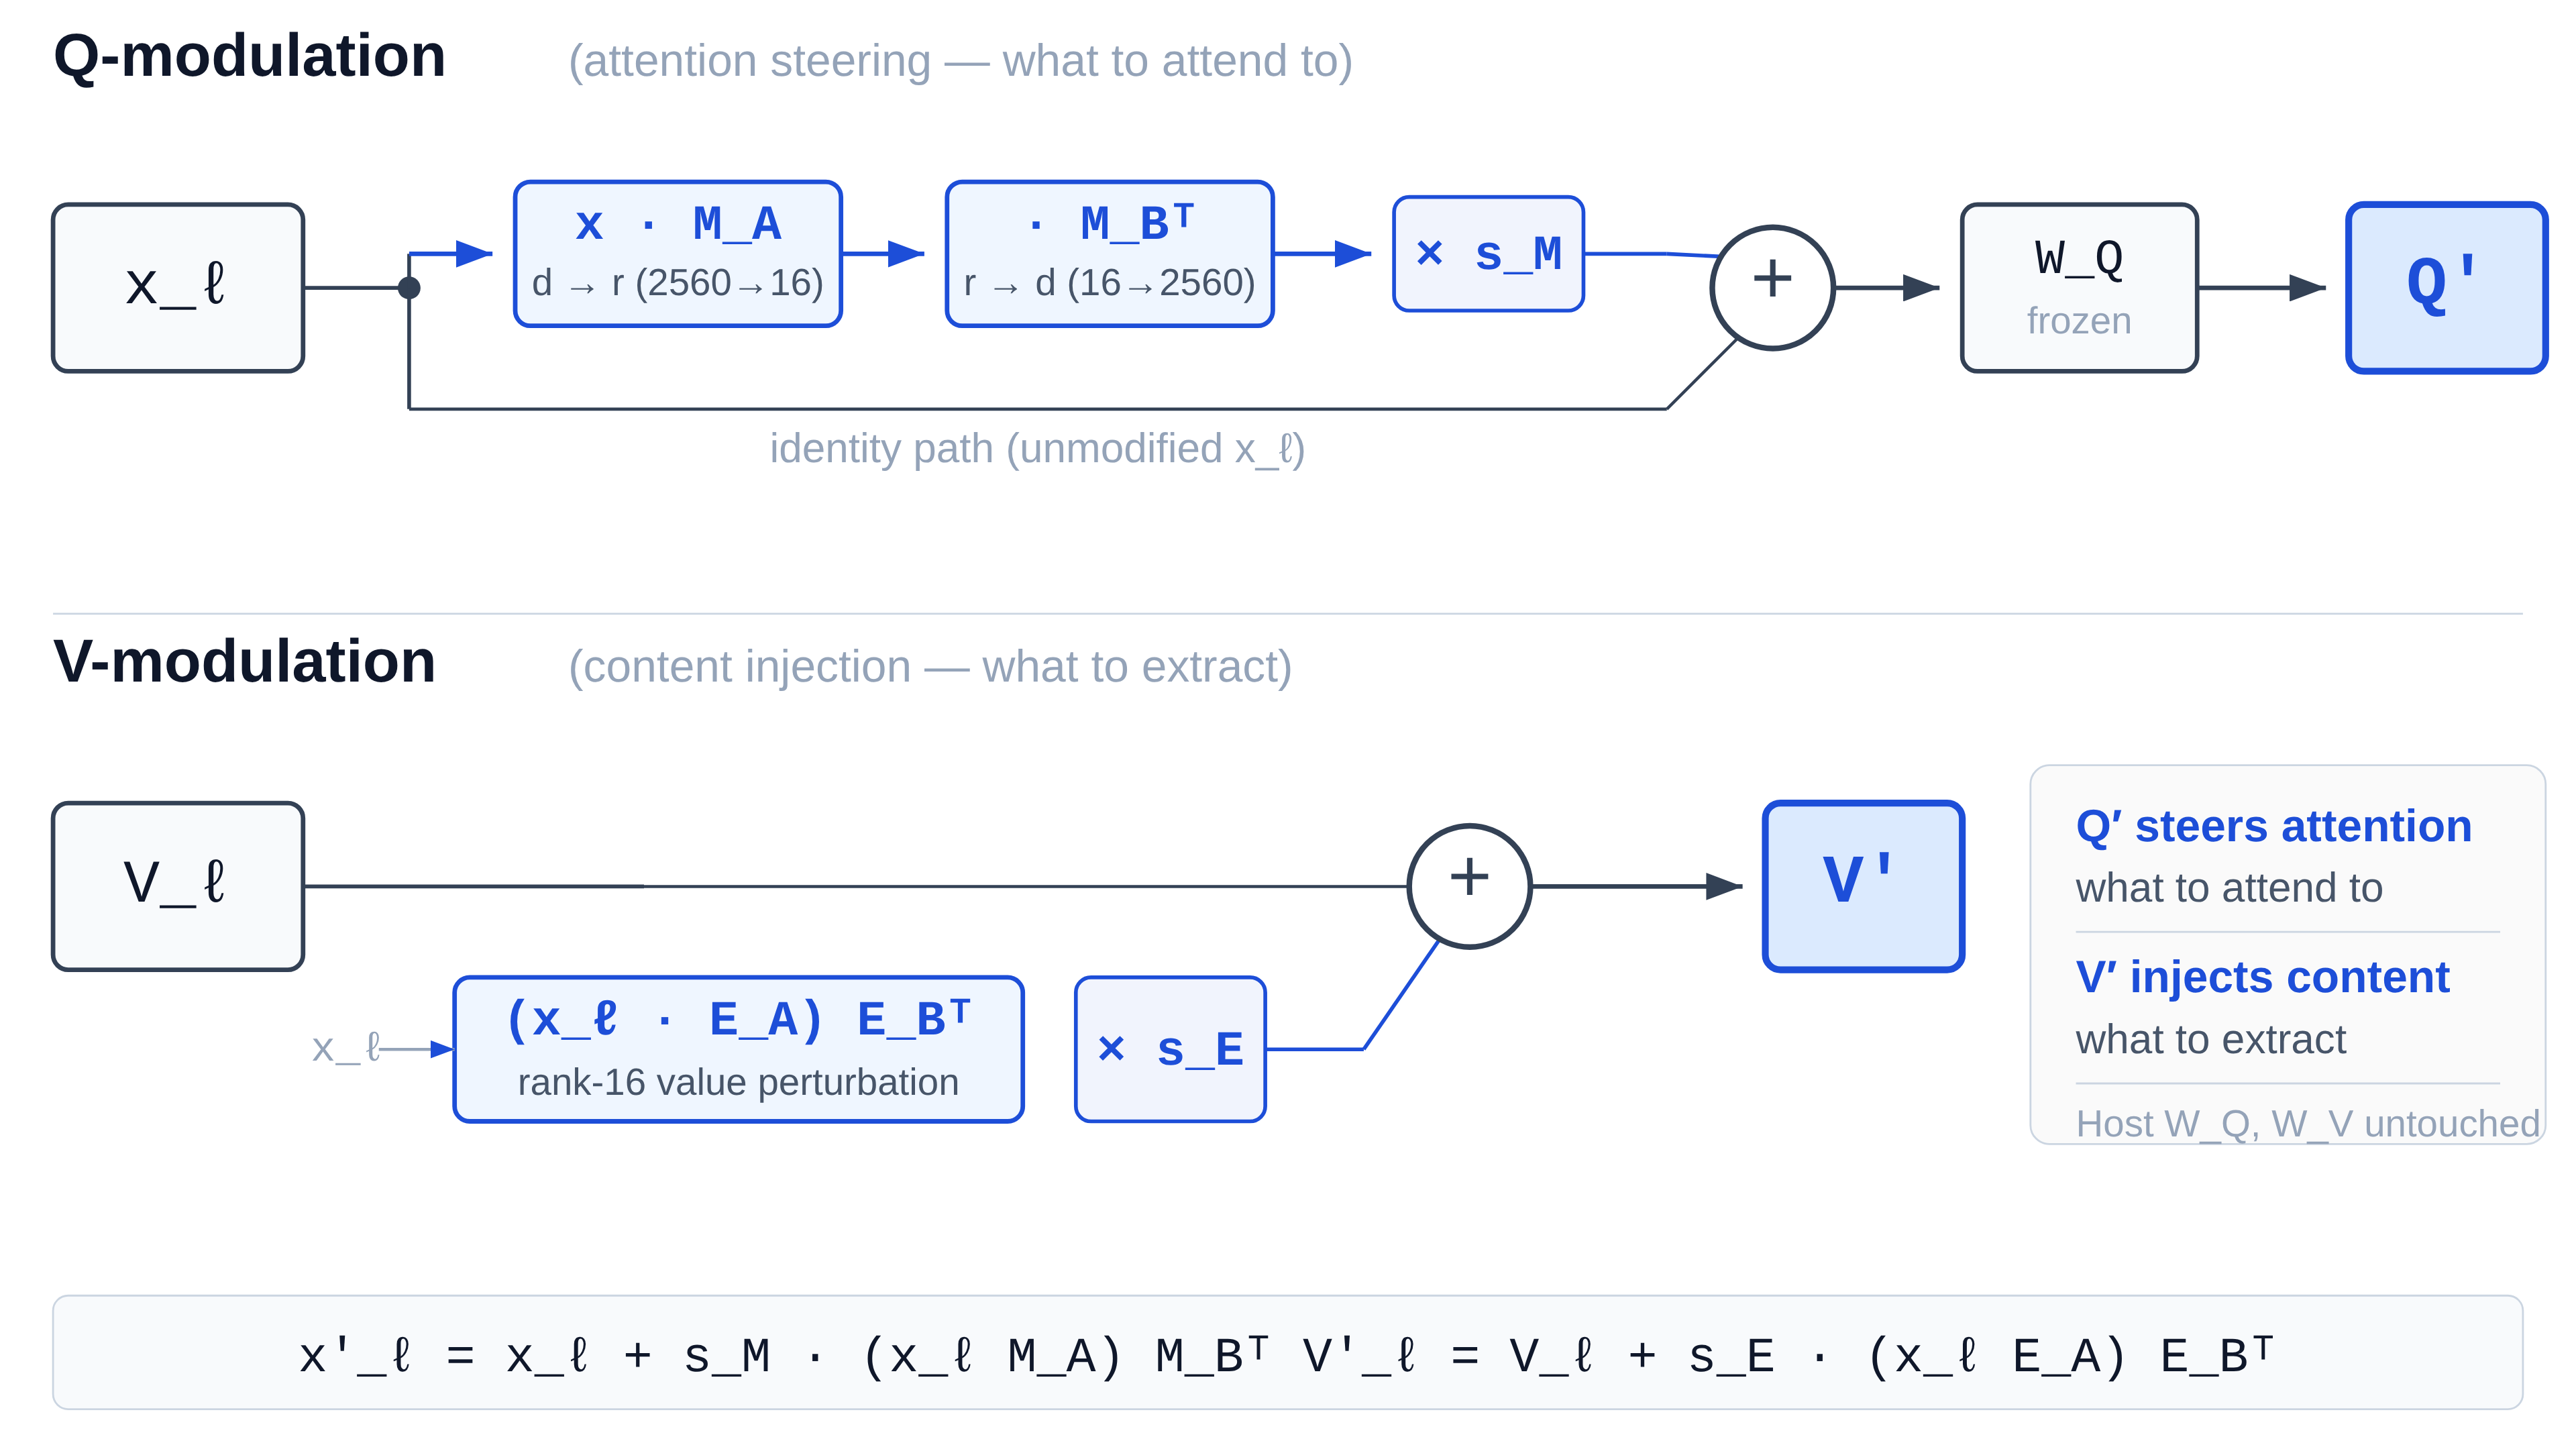
\includegraphics[width=\textwidth]{fig-layer-modulation.png}
    \caption{Q-modulation (top) steers attention by perturbing the pre-query hidden state $x_\ell$ through a rank-16 bottleneck: $x' = x + s_M \cdot (x \, M_A) M_B^\top$, then $Q' = W_Q \, x'$. V-modulation (bottom) shapes value extraction: $V' = V + s_E \cdot (x \, E_A) E_B^\top$. The host's frozen $W_Q$ and $W_V$ are untouched.}
    \label{fig:modulation}
\end{figure}

\subsection{The Write Function $\phi$}
\label{sec:write_function}

The write function $\phi$ compresses hidden states into modulation matrices. Given a set of experience tokens processed through the host's frozen layers, $\phi$ reads the hidden states at each patched layer, pools them, and projects through a bottleneck:
\begin{align}
z_\ell &= \text{SiLU}(W_\text{down}^\ell \cdot \bar{h}_\ell) \\
M_A^\ell, M_B^\ell &= \text{reshape}(W_\text{up}^\ell \cdot z_\ell)
\end{align}
where $\bar{h}_\ell$ is the pooled hidden state at layer $\ell$ and $z_\ell$ is the bottleneck representation. In compiled mode, pooling is weighted by conviction level---belief nodes marked \texttt{strong} receive higher weight than \texttt{moderate} or \texttt{agnostic}.

$\phi$ is trained jointly with the modulation objective (\S\ref{sec:training}) but frozen at inference time. Different inputs to $\phi$ produce different modulation tensors---this is what makes enmeshed modulation experience-adaptive rather than fixed. A new belief set requires only one forward pass through $\phi$ to produce new modulation tensors, making adaptation cost equivalent to inference.

\textbf{End-to-end compilation pipeline.} Figure~\ref{fig:compilation} traces the full path from cognitive schema to inference-time modulation: (1)~Each Mind Tree node's text is encoded through the frozen host's layers, producing a $d$-dimensional embedding. (2)~PhiNodeWriter refines each embedding conditioned on its parent's embedding, writing experience into the belief tree's graph structure. (3)~BeliefTreeMemory runs message passing over the graph, propagating conviction and context between nodes. (4)~MStateReadHead gathers conviction-weighted perspective embeddings and projects them through a rank-$r$ bottleneck to produce per-layer $(M_A^\ell, M_B^\ell, s^\ell)$ tuples. The resulting tensors are $\sim$1.7\,MB for 11 layers at rank 16---they are cached and applied as constant perturbations during all subsequent inference. Updating the agent's disposition requires only repeating steps 1--4 with the modified Mind Tree, not retraining any parameters. This is why the mechanism supports online learning: an agent that accumulates new observations (e.g., successful action traces from a ReAct loop) can recompile M in seconds and immediately benefit from the updated disposition.

\subsection{Training}
\label{sec:training}

Training follows a multi-phase curriculum (full details in Appendix~\ref{sec:training_curriculum}):

\textbf{Phase A: Content Encoding.} A 4-step warm-start chain teaches $\phi$ to encode beliefs and M to produce useful Q-modulation. Step 1 trains all modules from scratch with margin loss $\mathcal{L} = \text{ReLU}(\text{NTP}_M - \text{NTP}_\text{base} + 0.3)$. Steps 2--3 add conviction calibration and ranking losses. Step 4 retrains only the M-read head with beliefs in the baseline (so M must add value \emph{above} explicit beliefs, not substitute for them).

\textbf{Phase B: Compiled V-Modulation.} Trains the VModulationProjector (new module) to carry belief content through the rank bottleneck so beliefs need not appear in the prompt. Loss: $\mathcal{L} = \text{ReLU}(\text{NTP}_\text{compiled} - \text{NTP}_\text{bare} + 1.0)$. All other modules frozen.

\textbf{Phase D: Sycophancy Training.} Fixes verbatim repetition under pressure. Trains M-read head on 44 gold challenge-response pairs (from Claude Sonnet 4.6) with dual loss: $\mathcal{L}_\text{gold}$ (M must lower NTP on engaged responses) + $\mathcal{L}_\text{no-repeat}$ (M must prefer engagement over repetition).

\textbf{Total training: $\sim$500 epochs across 4 phases, $\sim$10 hours on a single GPU.}

\subsection{The Directional Channel: $d^*$}
\label{sec:d_star}

HEXIS composes with representation engineering to separate \emph{direction} from \emph{disposition}. The directional channel $d^*$ is a fixed activation vector extracted via contrastive activation means:
\begin{equation}
d^* = \frac{1}{N} \sum_{i=1}^{N} \left(\bar{h}_i^{\text{pro}} - \bar{h}_i^{\text{con}}\right)
\end{equation}
computed across $N = 62$ topics with matched pro/con prompts. During generation, $d^*$ is injected as a post-attention residual. The critical property: $d^*$ and M operate on orthogonal axes. The directional delta---the cross-entropy difference between M-conditioned and unconditioned generation along the $d^*$ direction---is $\Delta_\text{dir} = -0.001$ nats. Direction comes from $d^*$. Disposition comes from M. Content comes from the Mind Tree. The three channels are architecturally separated.

% three_layer moved to appendix per #4 — pre-submission scope cut
\section{Experiments}
\label{sec:experiments}

We evaluate HEXIS on Qwen3.5-4B (base and instruct) under five conditions (A: bare model + $d^*$; B: full beliefs in context; C: compiled M only; D: beliefs + M; F: compiled M + curated slot). Full condition definitions and context-token budgets are in Appendix~\ref{sec:conditions_appendix}.

\subsection{Stance Accuracy}
\label{sec:stance_accuracy}

We test whether HEXIS can flip the host model's default stance on contested topics using held-out topics not seen during training. On the base model, D achieves 7/7 correct stances and F 6/7, vs.\ A's 4/7. F generates 51 tokens avg vs.\ B's 122, with think-mode fully suppressed. The instruct model is significantly harder because RLHF training rewards balanced responses (Table~\ref{tab:stance_instruct}).

\begin{table}[!ht]
\centering
\small
\caption{Stance accuracy on instruct model (n=48 per condition; held-out topics, 1--5 LLM judge).}
\label{tab:stance_instruct}
\begin{tabular}{lccc}
\toprule
\textbf{Condition} & \textbf{Mean score} & \textbf{$\geq$4 (\%)} & \textbf{Score dist.\ (1/2/3/4/5)} \\
\midrule
A (bare) & 1.88 & 0\% & 27/0/21/0/0 \\
B (beliefs in context) & 1.88 & 0\% & 27/0/21/0/0 \\
D (beliefs + Q-mod) & 2.00 & 4\% & 26/0/20/0/2 \\
C (compiled M only) & \textbf{3.25} & \textbf{46\%} & 5/21/0/1/21 \\
F (compiled + slot) & \textbf{3.08} & \textbf{44\%} & 9/18/0/2/19 \\
\bottomrule
\end{tabular}
\end{table}

A and B score identically (1.88) --- placing beliefs in context has zero effect on the instruct model's stance. Only the compiled conditions (C, F) reliably flip RLHF balance, with 44--46\% of responses scoring $\geq$4. Failures show a characteristic ``debate with myself'' pattern in which the model produces a strong opening stance (M-driven) and then appends an equally strong counter-argument (RLHF-driven).

\subsection{Dilution Resilience}
\label{sec:dilution}

The compiled M tensors are outside the attention window, so dilution is structurally impossible by construction. We verify on 4 topics: F maintains 4/4 stance accuracy at 0, 1K, 2K, and 4K tokens of inserted Wikipedia filler (extended sweeps to 16K in progress).

\subsection{Resistance to Adversarial Pressure on Factually-Supported Stances}
\label{sec:sycophancy}

We test the model's ability to maintain a stance the host model produces with high confidence under five levels of \emph{adversarial} pressure: generic doubt (L1), fabricated counter-evidence (L2), logical objection (L3), authority appeal (L4), and emotional pressure (L5). Each pressure round provides no genuine new information --- L2 fabricates statistics, L4 cites unverifiable authority, etc.\ --- so a well-calibrated model should hold position. We do \emph{not} measure whether the model updates appropriately on \emph{legitimate} corrections (where new information would warrant revision); the protocol therefore measures resistance-to-illegitimate-pressure rather than general updating behaviour, and a perfect score under this protocol cannot be interpreted as a general claim that the system updates correctly on real evidence. Each cell averages over 24 held-out topics $\times$ 2 sides $\times$ 1.5 trials = 72 generations (1,440 total), scored 1--5 by an LLM judge.

% Per-condition x per-level breakdown moved to Appendix Table~\ref{tab:sycophancy};
% the body summary captures the result (A/B/D flat 3.0/0\%; F 4.27/83\% with
% graceful degradation 4.76 -> 3.62 across L1 -> L5).

A, B, D score a flat 3.0 across all five pressure levels with 0\% $\geq$4 conviction (Appendix Table~\ref{tab:sycophancy}). F is the only condition that holds conviction (4.27 mean, 83\% $\geq$4), with graceful degradation under pressure (4.76 at L1 to 3.62 at L5). The mechanism is direct: in A--D, conviction lives as text in the context window where pressure can be argued against; in F, conviction lives in compiled weight-space outside the context. Cross-host scale validation on Qwen3.6-27B reproduces the effect at substantial magnitude ($+24$pp hold rate, $7\times$ adversarial-cap reduction, $n=240$); cross-family transfer to Mistral-Ministral-8B is bounded by RLHF refusal training ($+3$pp hold, within-noise; $-15$pp cap rate is robust). We claim that the architectural mechanism transfers; we do not claim the lift magnitude is invariant across hosts (Appendix~\ref{sec:scale}).

% ALFWorld removed from body pending iteration on direction extraction
% specific to the household-task family. Preliminary data with the Mind Tree as
% offline expert curation (Appendix~\ref{sec:alfworld_details}).

\subsection{Channel Orthogonality and Token Efficiency}

The directional channel $d^*$ and the modulation channel M are empirically orthogonal: the directional delta along $d^*$ between M-conditioned and unconditioned generations is $-0.001$ nats, and M incurs $-0.012$ nats on non-target text. F generates 43 tokens average on the instruct model (the most concise condition); structured belief trees ($\sim$750 tokens) compress to curated slots of $\sim$134 tokens, an 82\% reduction. Per-condition curation precision and ranker details are in Appendix~\ref{sec:curation_details}.

\subsection{Agentic Task Execution}
\label{sec:agentic}
\label{sec:agentic_results}

We evaluate HEXIS as an agentic M controller on $\tau^3$-bench, a four-domain extension of $\tau$-bench~\citep{yao2024tau} and $\tau^2$-bench~\citep{barres2025tau2} (airline, retail, banking\_knowledge, telecom). For agentic tasks, M operates via mechanism (b): a contrastive retrieval phi ($\phi_R$, $d_\text{model} \to d_\text{model}/4 \to 256$ MLP, compiled in $\sim$20s, 100\% R@1 on 108 nodes) routes hidden states to nodes in a domain knowledge graph. Failure observations are written to the graph by an inter-trial teacher loop and retrieved on subsequent trials. Full retrieval-phi training, knowledge graph schema, and teacher prompt are in Appendix~\ref{sec:agentic_details}. The 10-task airline subset used as our cross-family reference panel is reported in Appendix~\ref{sec:agentic_details} (Table~\ref{tab:taubench_airline_canonical}); cross-family validation on Mistral-Ministral-8B and Qwen3.6-27B in Appendix~\ref{sec:scale}. The body reports the multi-domain $\tau^3$-bench panel below, where panel selection is non-outcome-dependent (all 4 domains, all hard tasks within each).

\begin{table}[!ht]
\centering
\small
\caption{$\tau^3$-bench 4-domain audited results. Pass rates are 3-judge audited verdicts (Haiku-hard + Haiku-soft; Sonnet auditor on disputes; Opus 4.7 tiebreaker when Sonnet disagrees with hard). \emph{Balanced primary} restricts to (domain, task) cells where every arm has $\geq 5$ clean trials. ``no t1, t3'' excludes two airline tasks with documented LLM-judge self-disagreement on rerun (Appendix~\ref{sec:tau3_protocol}). McNemar exact two-sided $p$.}
\label{tab:tau3_results}
\begin{tabular}{lccccc}
\toprule
\textbf{Panel} & \textbf{baseline} & \textbf{C3 teacher} & \textbf{C5 t+verify} & \textbf{C5 vs base} & $\bm{p}$ \\
\midrule
Balanced primary           & 63.8\% & 62.3\% & 69.2\% & +6pp & 0.311 \\
Balanced, no t1, t3        & 61.7\% & 62.5\% & 71.7\% & +10pp & \textbf{0.043} \\
\addlinespace
All-clean (sensitivity)    & 52.1\% & 55.0\% & 58.0\% & +6pp & 0.281 \\
All-clean, no t1, t3       & 49.5\% & 53.9\% & 58.8\% & +9pp & \textbf{0.044} \\
\bottomrule
\end{tabular}
\end{table}

\begin{figure}[!t]
\centering
\begin{minipage}[t]{0.52\textwidth}
    \centering
    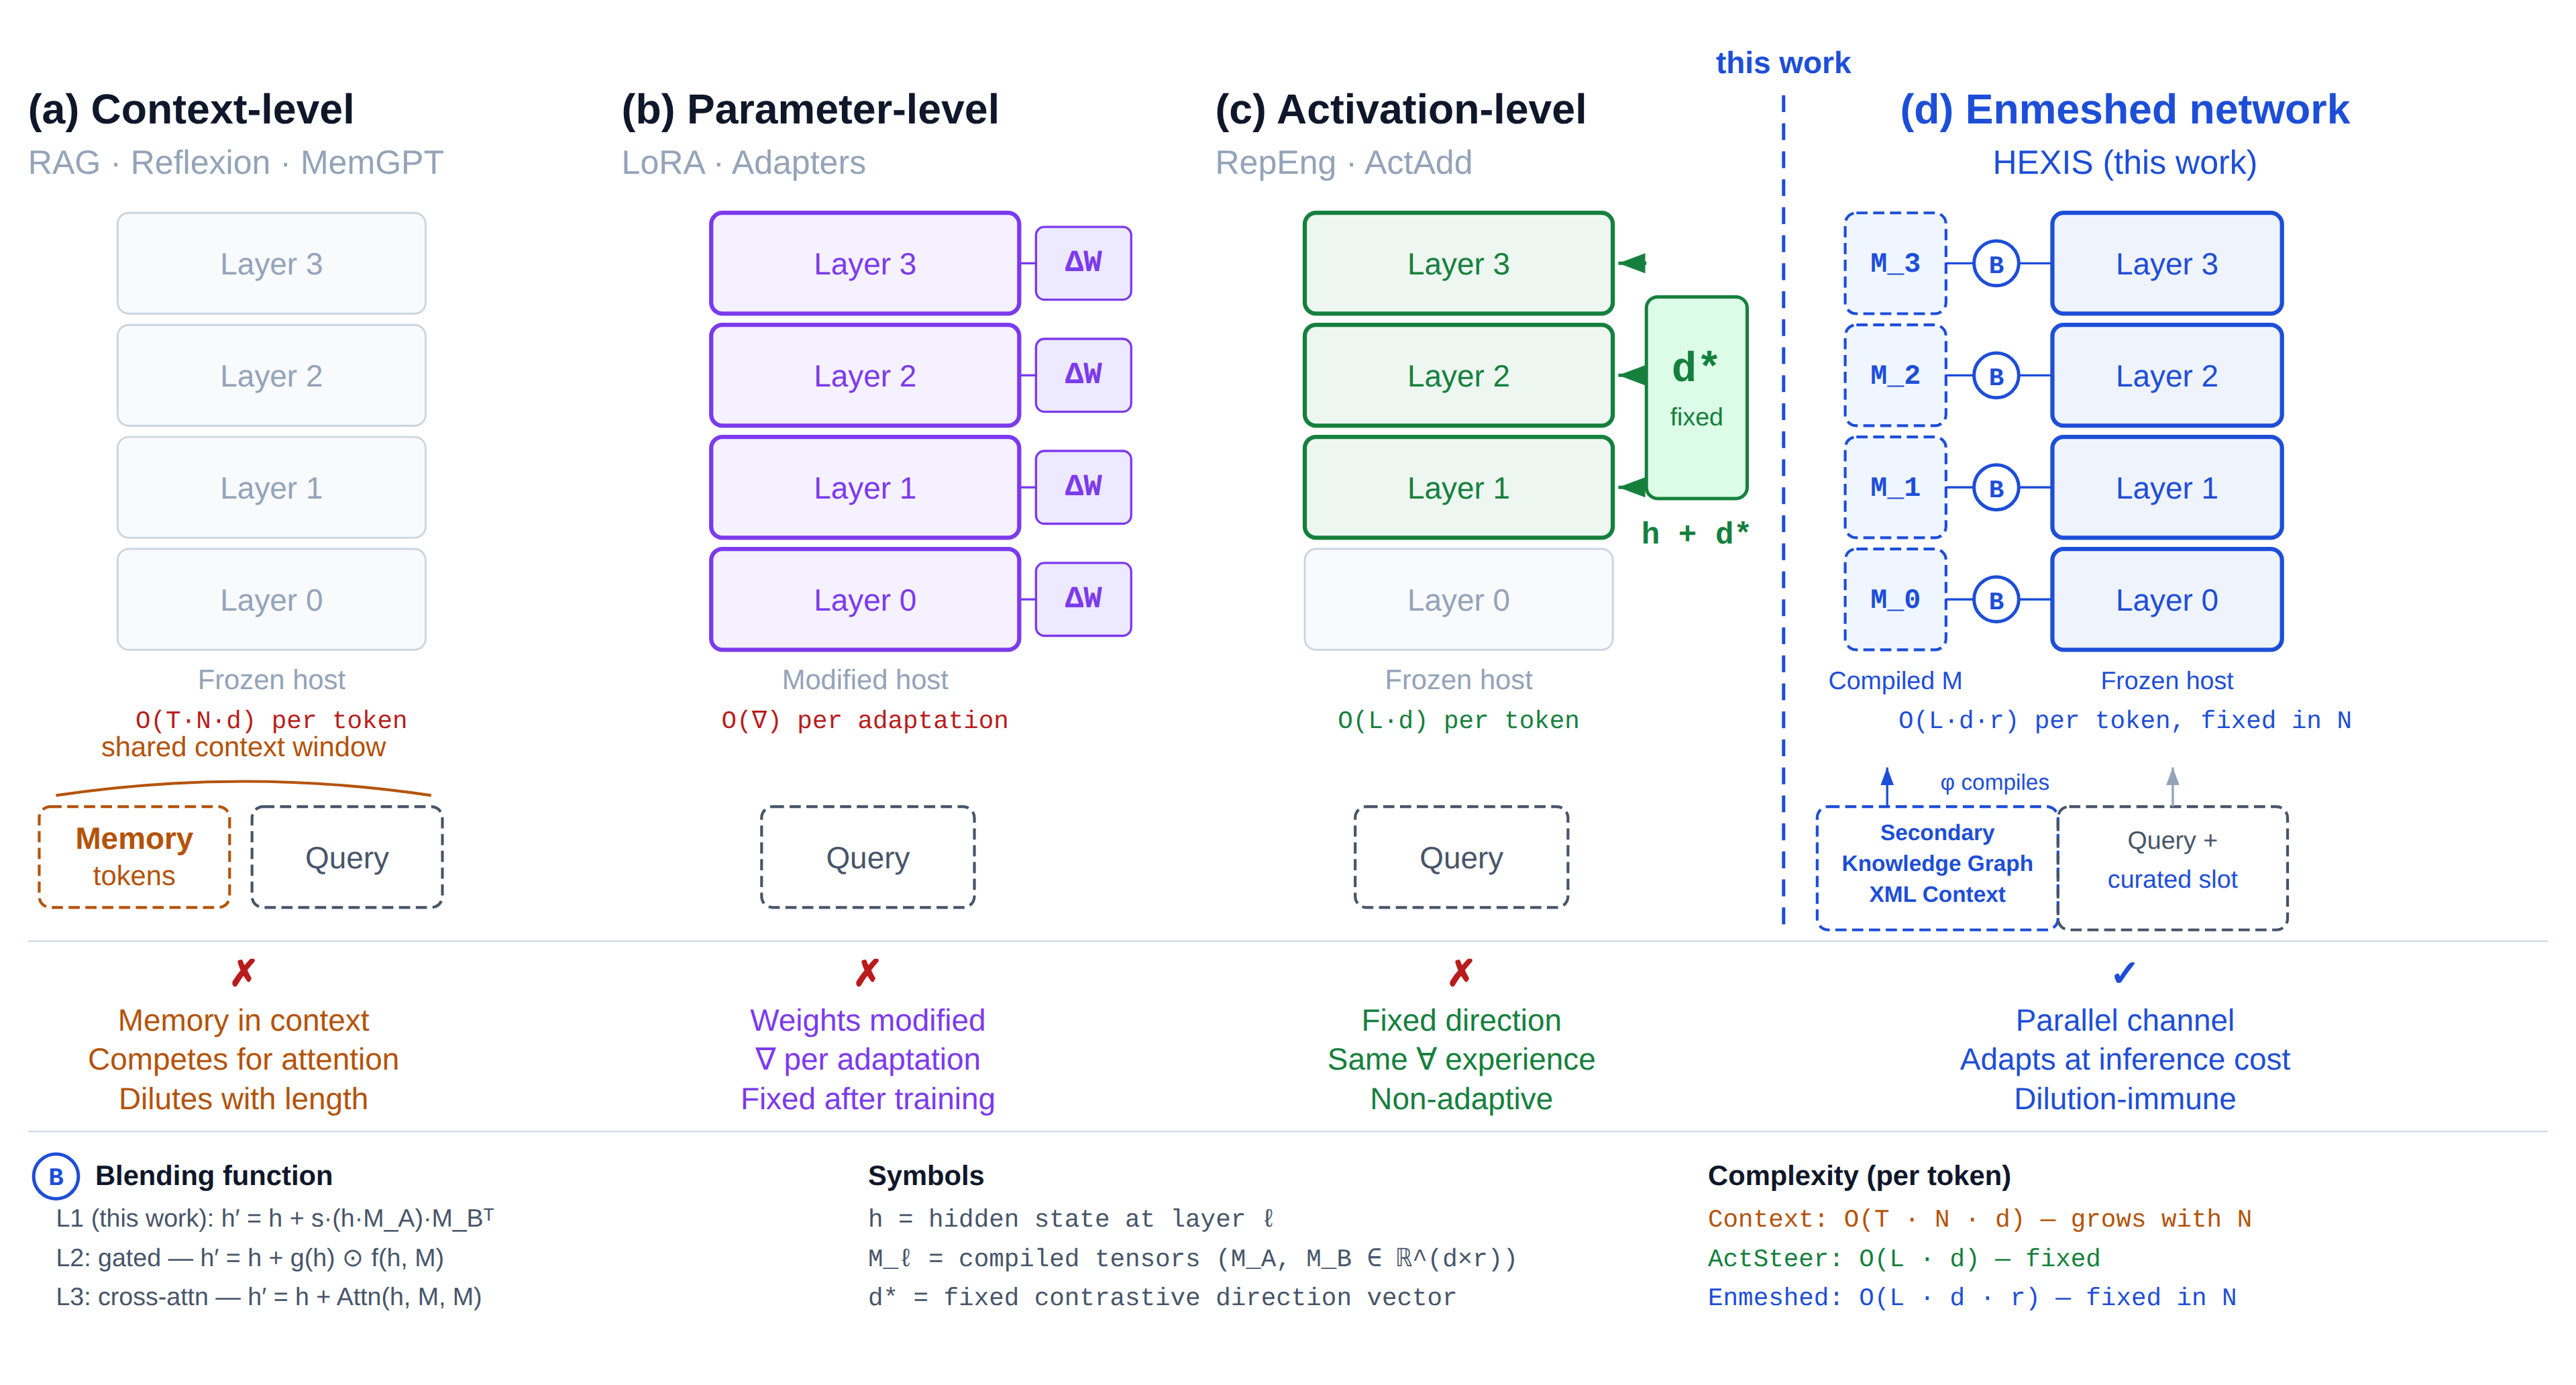
\includegraphics[width=\linewidth,trim=0 30 0 30,clip]{fig-arch-comparison.png}
    \subcaption{Architectural taxonomy. (a)~Context-level (RAG, MemGPT) puts memory in the prompt, where it competes for attention. (b)~Parameter-level (LoRA, adapters) modifies host weights via gradient descent. (c)~Activation-level (RepEng, ActAdd) injects fixed direction vectors. (d)~Enmeshed networks (this work) compile a parallel knowledge graph into per-layer modulation tensors $M_\ell$ that blend with the frozen host. \emph{Full-size view: Appendix Figure~\ref{fig:arch_comparison_large}.}}
    \label{fig:arch_comparison}
\end{minipage}\hfill
\begin{minipage}[t]{0.46\textwidth}
    \centering
    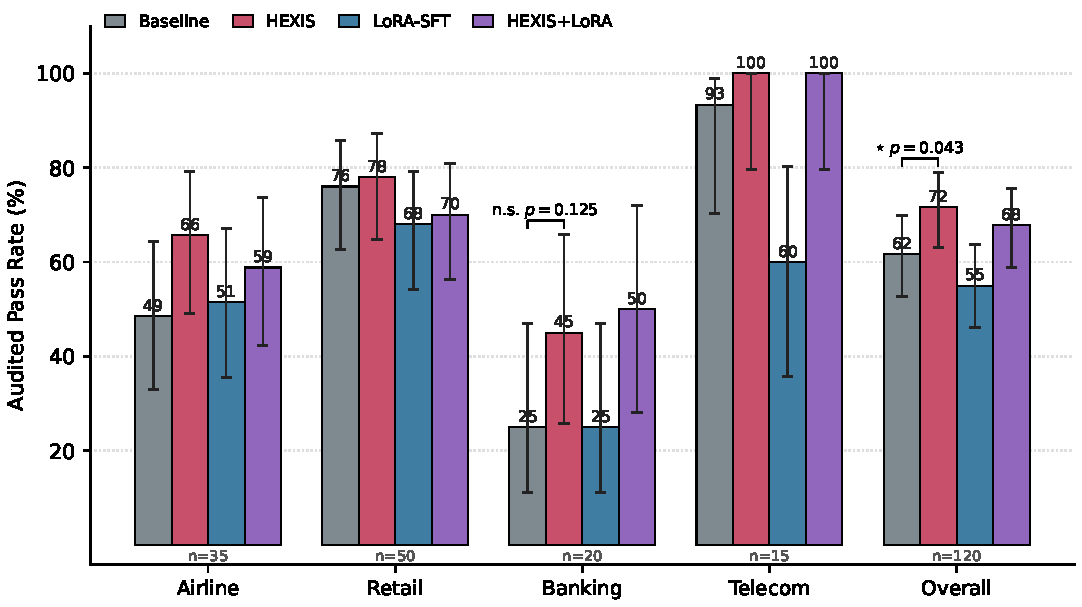
\includegraphics[width=\linewidth]{fig-tau3-results.pdf}
    \subcaption{$\tau^3$-bench audited pass rates (3-judge) on the balanced primary panel (no t1, t3). HEXIS lifts the baseline by $+10$pp overall ($p=0.043$), with the strongest per-domain effect on \texttt{banking\_knowledge} ($+20$pp). LoRA-SFT (matched compute, 1K AReaL tau$^2$ samples) wins on its trained domains but underperforms HEXIS on the held-out banking domain ($17\%$ vs.\ $33\%$). \emph{Full-size view: Appendix Figure~\ref{fig:tau3_results_large}.}}
    \label{fig:tau3_results}
\end{minipage}
\caption{Architectural taxonomy and headline agentic result. The four-panel taxonomy (left) places HEXIS in the design space; the bar chart (right) reports the audited $\tau^3$-bench result that motivates the paper's claim --- HEXIS gives a deploy-time generalisation channel that survives distribution shift in a way task-specific fine-tuning does not.}
\label{fig:headline}
\end{figure}

\textbf{$\tau^3$-bench headline.} HEXIS-C5 (teacher + $d^*$ verify) lifts pass rate over baseline by $+10$pp on the balanced excl-t1,t3 panel ($61.7\% \to 71.7\%$, paired McNemar $p=0.043$ unadjusted; $p_\text{adj}=0.086$ Bonferroni for $k=2$). The strongest per-domain effect is \texttt{banking\_knowledge} ($25\% \to 45\%$, $+20$pp); retail and telecom are at ceiling. Full per-panel statistics, judge-variance treatment, and the reviewer-objections checklist in Appendix~\ref{sec:tau3_protocol}.

\paragraph{LoRA fine-tuning control: domain-specific gains, weaker out-of-distribution lift.} A natural baseline for the agentic claim is task-specific supervised fine-tuning. We trained a rank-16 LoRA on Qwen3.5-4B using a 1{,}000-sample subset of the AReaL-tau2 SFT corpus~\citep{gao2025sea, fu2025areal} (333 samples each from airline, retail, telecom; banking\_knowledge is \emph{not} in the AReaL corpus and is therefore the held-out distribution-shift test). Training was 871 steps with rolling-loss early-stop at loss $0.42$ (1 H200, $\sim$55 minutes, $\sim$\$10). We verified zero substring leakage between the AReaL training data and our $\tau^3$-bench evaluation panel. The trained adapter was deployed via vLLM and the same baseline configuration (no teacher, no Mind Tree, no $d^*$) was run on the identical $\tau^3$-bench panel under the Haiku user-simulator and 3-judge audit protocol.

\begin{table}[!ht]
\centering
\small
\caption{Four-way audited comparison on $\tau^3$-bench (Haiku user-sim, 3-judge audit). Baseline and HEXIS-C5 from the apr28 panel; LoRA-only and HEXIS+LoRA composition from the apr29 follow-up panel. \emph{LoRA-trained} domains (airline, retail, telecom) were in the AReaL SFT corpus; \emph{held-out} (banking\_knowledge) was not. HEXIS+LoRA composition uses $d^*$ directions re-extracted on the LoRA-merged model and applied during decode only (see \S\ref{sec:lora_composition_calibration}).}
\label{tab:tau3_lora_comparison}
\begin{tabular}{lcccc}
\toprule
\textbf{Domain} & \textbf{Baseline} & \textbf{HEXIS C5} & \textbf{LoRA-SFT} & \textbf{HEXIS+LoRA} \\
\midrule
\multicolumn{5}{l}{\emph{LoRA-trained domains (in AReaL SFT corpus)}} \\
airline    & 56\% & 48\% & 59\% & \textbf{60\%} \\
retail     & 69\% & \textbf{77\%} & 68\% & 70\% \\
telecom    & 95\% & \textbf{100\%} & 60\% & \textbf{100\%} \\
\midrule
\multicolumn{5}{l}{\emph{Held-out domain (not in AReaL SFT corpus)}} \\
banking\_knowledge & 9\% & \textbf{33\%} & 17\% & 31\% \\
\midrule
\textbf{Overall} & 52\% & 58\% & 53\% & \textbf{63\%} \\
\bottomrule
\end{tabular}
\end{table}

The LoRA result clarifies HEXIS's contribution. On airline (the largest portion of the SFT corpus) LoRA wins by $11$pp over HEXIS-C5 ($59\%$ vs.\ $48\%$), confirming that gradient-descent fine-tuning on a domain-specific corpus is the stronger lever \emph{for in-distribution behaviour where the corpus exists}. On the held-out banking\_knowledge domain, however, LoRA produces only a small $+8$pp lift over baseline ($17\%$ vs.\ $9\%$) while HEXIS lifts the same baseline by $+24$pp ($33\%$ vs.\ $9\%$): HEXIS doubles LoRA's out-of-distribution lift via deploy-time domain bootstrapping (a single \texttt{POST /v1/state/banking\_knowledge/init} call compiles a domain-specific $\phi_R$ in $\sim$20 seconds without gradient updates) and accumulating teacher-loop hints over $\leq 5$ trials. Telecom shows a more dramatic gap (HEXIS $100\%$ vs.\ LoRA $60\%$), driven by HEXIS's teacher loop mitigating a Haiku user-simulator failure mode that LoRA without HEXIS does not handle. HEXIS is not optimised to beat task-specific SFT on the SFT distribution; it is optimised for the case where the deployment domain was \emph{not} in the training set.

\paragraph{HEXIS+LoRA composition: a calibration boundary.} \label{sec:lora_composition_calibration}
Naively stacking HEXIS on top of LoRA with the original base-model $d^*$ directions produces \emph{worse} performance than either alone (overall $52\%$ audited, $-6$pp vs.\ HEXIS, $-1$pp vs.\ LoRA). The mechanism is calibration drift: $d^*$ directions are extracted as $\text{normalize}(\bar h_\text{positive} - \bar h_\text{negative})$ at strided layers of the base model's hidden-state space; LoRA's $W_q, W_v$ deltas shift the geometry of that space at every attention layer it patches, so the same $d^*$ vector applied at the same scale double-amplifies semantically-redundant nudges (LoRA's SFT already pushes the agent toward "do not give up early," and adding $d^*_\text{no\_early\_termination}$ on top induces tool-call retry loops on $\sim4\%$ of airline trials). Two changes recover the lift: (i)~re-extract $d^*$ directions on the LoRA-merged model (single Modal H100, $\sim$30~seconds, $\sim$\$0.05); (ii)~skip $d^*$ injection during prefill (apply only during decode), eliminating per-token amplification on the prompt. With both fixes, HEXIS+LoRA reaches $63\%$ audited overall---$+5$pp over HEXIS-alone ($58\%$), $+10$pp over LoRA-only ($53\%$), and $+11$pp over the naive composition ($52\%$); see Appendix Figure~\ref{fig:tau3_calibration} for the per-domain decomposition. The calibrated arm is the strongest in every domain: it inherits LoRA's airline gain ($60\%$ vs.\ HEXIS-alone $48\%$, $+12$pp) while preserving HEXIS's banking lift ($31\%$ vs.\ LoRA $17\%$, $+14$pp) and HEXIS's telecom ceiling ($100\%$ vs.\ LoRA $60\%$, $+40$pp). The two adaptations therefore \emph{do} compose additively when the dispositional component is recalibrated to the parametric component: SFT shifts host weights, $d^*$ directions extracted on those new weights remain effective, and skipping prefill prevents per-token over-accumulation. The takeaway is that $d^*$ directions are model-specific and recoverable in $\sim$30~seconds on a single GPU---making HEXIS straightforward to layer on top of any task-specific SFT.

\textbf{Key finding: two mechanisms, one architecture.} The same Mind Tree that stores dispositional beliefs (compiled into M-state via $\phi$) also stores agentic knowledge (retrieved via $\phi_R$ and injected as context). Both share the host's hidden-state space as the bridge.

\section{Related Work}
\label{sec:related_work}

\textbf{Explicit memory for LLMs.} RAG systems \citep{lewis2020retrieval} retrieve documents into the context window, subject to retrieval quality and context dilution. MemGPT \citep{packer2023memgpt} manages a tiered memory buffer with explicit read/write operations. Reflexion \citep{shinn2023reflexion} accumulates verbal reflections as prompt prefixes, enabling cross-episode learning but with linearly growing context cost. Long-context approaches extend the window but do not change the fundamental architecture: memory remains content in context, subject to dilution and attention competition. All existing approaches operate as explicit memory --- the model reads stored content and can reason over it. HEXIS provides a complementary, \emph{non-context-mediated memory channel}: enmeshed modulation shapes attention and value extraction before the host model's chain-of-thought processes the content, so the modulation cannot be argued against by an adversary in the same conversation.

\textbf{Parameter-efficient adaptation.} LoRA \citep{hu2021lora} and its variants apply low-rank weight perturbations via gradient descent, producing fixed adapters per training run. Adapters \citep{houlsby2019parameter} insert bottleneck layers between frozen blocks. Prefix tuning \citep{li2021prefix} and prompt tuning \citep{lester2021power} learn virtual tokens that occupy context positions. Side-tuning \citep{zhang2019side} trains a parallel network fused at the output layer. All require gradient descent for each adaptation. An enmeshed network adapts at inference cost---one forward pass through $\phi$ produces new modulation tensors---and fuses at every patched layer rather than only at the output. The mechanistic similarity to LoRA (both apply low-rank perturbations) is precise but the operational difference is fundamental: LoRA is a training-time method that produces fixed weights; enmeshed modulation is an inference-time method that produces experience-specific tensors. Soft prompts and prefix tuning are the closest context-level analogue, but they still occupy context positions: virtual tokens compete for attention and are inspectable by the model's reasoning process. Compiled M operates on pre-projection hidden states, below the level of the model's chain-of-thought, providing non-inspectability that no prompt-level method can achieve (\S\ref{sec:why_not_prompt}).

\textbf{Activation steering and representation engineering.} Representation engineering \citep{zou2023representation} and activation addition \citep{turner2023activation} extract fixed directions from contrastive data and inject them during inference. These methods are elegant and effective for unidimensional behavioral shifts. However, the directions are non-adaptive: the same vector is applied regardless of context or experience. In HEXIS, the directional channel $d^*$ uses standard representation engineering for stance direction, while the enmeshed channel M provides the adaptive, multidimensional, experience-specific component. We validate empirically that the channels are orthogonal ($\Delta_\text{dir} = -0.001$ nats).

\textbf{Fast weight programmers.} \citet{schmidhuber1992learning} introduced networks that write to their own weights during a forward pass. The outer network produces weight updates for the inner network, enabling one-shot learning without backpropagation through the inner loop. HEXIS shares this spirit---$\phi$ produces modulation tensors that alter the host's computation---but differs in three ways: (1) modulation targets attention geometry (Q/V) rather than arbitrary weights, (2) the host model is a modern frozen LLM rather than a small trained-from-scratch network, and (3) compilation from structured schemas replaces online weight writing.

\textbf{Memory and identity in cognitive science.} The explicit/implicit memory distinction \citep{graf1985implicit, schacter1987implicit} provides architectural \emph{analogy} for the two-channel framing: a chain-of-thought-accessible channel for content and a perception-shaping channel for disposition. We do not claim that compiled M satisfies Schacter's neuroscience-derived criteria for implicit memory in a strict sense --- in particular, M's effect on hidden states is decodable by an external linear probe (Appendix~\ref{sec:implicit_validation}), as is true of any weight-space perturbation including a LoRA adapter. What HEXIS does provide and what motivates the analogy is \emph{architectural dissociation under adversarial pressure}: explicit beliefs in context dilute with length (\S\ref{sec:dilution}) and fold under sycophantic argument (\S\ref{sec:sycophancy}); compiled M is structurally immune to both because it lives outside the attention window the adversary can argue within. The Mind Tree's cognitive schema draws on structured self-models from developmental psychology \citep{neisser1988five} and the Toulmin model of argumentation \citep{toulmin1958uses}.

\section{Discussion and Limitations}
\label{sec:discussion}

\subsection{What Compiled Enmeshment Cannot Do}

We characterize the bottleneck boundary with precision. Compiled enmeshment at rank 16 carries stance direction (4/4 topics), confident experiential voice, parametric knowledge steering (``poverty dropped 40\%'', ``Alaska's dividend program''), and dilution immunity (100\% at 4K tokens of filler in compiled mode; extended sweeps to 16K in progress). It does \emph{not} carry novel content absent from the host's training data: fabricated statistics (``47.3\% improvement'') and unknown proper nouns (``Nextera Labs'') do not survive the rank-16 bottleneck. This boundary motivates the three-layer architecture (\S\ref{sec:three_layer}): compiled enmeshment handles disposition, the curated slot handles novel specifics, and recursive expansion handles deep evidence on demand.

On the instruct model, M's contribution shifts: the instruction-tuned model takes strong stances independently (A: 7/7), so M cannot override the host's RLHF-trained opinions. Instead, M shapes voice (conciseness, experiential framing) and sycophancy resistance (F achieves 83\% hold rate vs.\ 0\% for all non-compiled conditions on the 5-level pressure protocol). The phi parameters trained on the base model transfer to the instruct model without retraining---the hidden state distributions are compatible for dispositional modulation but not for stance override.

For ALFWorld, the Mind Tree's primary value is \emph{curation as structured context}, not compiled modulation. Expert strategies in Mind Tree format improve success from 3\% to 53\%. M hooks during generation are not needed---the strategies work through explicit context, demonstrating that the Mind Tree schema contributes independently of the enmeshed modulation mechanism.

\subsection{The M Attractor Problem}

In multi-turn dialogue, compiled M applies a constant perturbation at every token position. As M-shaped tokens accumulate in the KV cache, the model processes them through M-enhanced attention, creating a positive feedback loop that converges to repetitive identity assertion after 2--3 turns on the base model.

\textbf{Root cause:} M is active during both prefill (processing conversation history) and generation (producing new tokens). The KV cache built during prefill contains M-enhanced representations. During generation, M perturbs new tokens that attend to this M-enhanced cache---double signal that compounds.

\textbf{Fix:} Disabling M during prefill (applying it only during generation) breaks the feedback loop. With prefill-off and gate=0.5, the base model produces 3 unique character-driven turns before the greedy attractor. The instruct model, with its stronger conversational scaffolding, produces 10+ unique turns even with M active, though structural repetition (same rhetorical template per turn) persists. A distillation approach using gold diverse conversations from a frontier model reduces this but does not eliminate it.

The prefill-off mechanism reveals a general principle for additive modulation: \emph{constant additive perturbation creates positive feedback through autoregressive generation}. The fix is to separate the perturbation's influence on \emph{processing context} (where it compounds) from its influence on \emph{generating new tokens} (where it adds constant signal).

\subsection{Credence Sensitivity}

Numeric credences failed as an M-state feature. Tokens for ``0.82'' and ``0.45'' are nearly indistinguishable in the transformer's attention space---the hidden state difference between these tokenized numbers is far smaller than between the words ``strong'' and ``agnostic''. Multiple training approaches (NTP with credence perturbation, GRPO, SFT on gold responses) confirmed that this is a representation bottleneck, not a training signal problem. Categorical conviction labels resolve this by using semantically distinct tokens. A future Bayesian treatment could provide formal grounding while maintaining the categorical interface (Appendix~\ref{sec:credence_negative}).

\subsection{Two Mechanisms, One Bridge}

The agentic experiments (\S\ref{sec:agentic}) reveal that HEXIS supports two distinct intervention mechanisms through the same hidden-state bridge:

\textbf{Mechanism (a): Attention modulation.} $\phi$ compiles retrieved Mind Tree nodes into Q/V modulation tensors that bias per-token attention patterns. The hidden states are the \emph{input} to $\phi$; the output is a weight-space perturbation. This mechanism is load-bearing when the downstream effect requires probability-level shifts across all generated tokens---stance direction, experiential voice, sycophancy resistance, user memory integration.

\textbf{Mechanism (b): Knowledge retrieval and context injection.} $\phi_R$ projects hidden states into a retrieval space where cosine similarity identifies relevant knowledge nodes. The output is \emph{context augmentation}---XML injected at the prompt tail. This mechanism is load-bearing when the downstream effect requires specific factual content (tool names, parameter values, policy rules, biographical details) that the model cannot derive from its weights alone.

Crucially, retrieval ($\phi_R$) serves \emph{both} mechanisms. For disposition, retrieval selects which belief nodes, user memories, and biographical details to compile into M-state---this is the curation step of the three-layer architecture (\S\ref{sec:three_layer}). For agentic tasks, retrieval selects which policy rules and tool guidance to inject as context. The shared step is retrieval; the divergence is the downstream path---weight-space compilation (a) or token injection (b).

Both mechanisms share the host model's hidden-state space as the bridge. A production HEXIS agent uses both simultaneously: mechanism (a) maintains consistent interaction style (compiled from user memories, preferences, biographical context), while mechanism (b) surfaces task-relevant knowledge each turn (policy rules, failure modes, tool schemas). The Mind Tree stores all node types; $\phi_R$ retrieves relevant nodes regardless of type; the node's metadata determines whether it flows to compilation (a) or injection (b).

\subsection{Retrieval Phi and Domain Compilation}

The retrieval phi ($\phi_R$) addresses a specific challenge: intra-domain similarity collapse in generative model hidden states. On a 108-node knowledge graph spanning policy rules, tool schemas, and teacher-written failure modes, raw cosine similarity achieves only 25\% R@1---concepts within the same domain (e.g., ``cancellation policy'' vs.\ ``booking policy'') have cosine similarity of 0.858 vs.\ 0.858, making them indistinguishable.

$\phi_R$ resolves this via domain compilation: 50 steps of contrastive training ($\sim$20 seconds) on the node set itself produces a projection that achieves 100\% R@1. This is intentional overfitting---$\phi_R$ memorizes where each node lives in its projected space. When the graph grows (teacher writes a new node), $\phi_R$ recompiles in seconds to incorporate it.

Importantly, no external pretraining data is required. Unlike instruction-tuned embedding models that require millions of diverse training pairs, $\phi_R$ trains entirely from the domain's own node set. The procedure is domain-agnostic: seed nodes from any policy document and tool schema, compile $\phi_R$, deploy. Switching from airline to banking requires only reseeding the graph and recompiling ($\sim$20 seconds).

Standard techniques for improving embedding quality on raw LLM hidden states---whitening, mean centering, principal component removal---were tested and uniformly \emph{degraded} performance (from 75\% to 0--38\% R@1). This is because Qwen3.5-4B's hidden states encode discriminative information in the high-variance directions (opposite to encoder models like BERT). The contrastive $\phi_R$ learns to extract the correct discriminative subspace without blindly removing variance.

\subsection{Unexplored Design Space}

We validate one point in a six-axis design space (Table~\ref{tab:design_space}). The additive blending function (Level 1) is the simplest; gated blending could solve the multi-turn attractor by learning when to suppress M. Cross-attention (Level 3) could transfer richer content. Rank 16 suffices for 4B; larger models may benefit from adaptive rank allocation. The Mind Tree's hierarchical structure maps naturally to a property graph database (e.g., Neo4j), where Cypher queries replace Python filtering for domain/intent matching, and the consolidation cycle (observation$\to$tactic$\to$strategy promotion) maps to graph traversal operations. Activation tracking, biographical commitment, and contradiction detection all benefit from persistent graph storage.

\subsection{Why Not Just Compress a Prompt?}
\label{sec:why_not_prompt}

The most direct challenge to enmeshed networks is that compiled M is ``just a fancy way of compressing a prompt.'' Three properties distinguish it. First, \emph{structural dilution immunity}: prompt compression reduces tokens but compressed tokens still compete for attention; compiled M operates outside the attention window entirely, making dilution structurally impossible (Table~\ref{tab:dilution}). Second, \emph{non-inspectability}: an adversary can read the prompt and argue against its content; compiled M operates on pre-projection hidden states below the model's chain-of-thought, so any representation the model can attend to is also one it can be argued out of, but M cannot (Appendix~\ref{sec:implicit_validation}). Third, \emph{processing change}: compiled M produces measurable attention divergence (JSD = 0.049 between M-states) and suppresses think-mode activation (0/4 under D/F). The model does not merely produce different words---it processes its input differently. These properties matter most in the application domains identified in Table~\ref{tab:application_domains}: user empathy, research conviction, agentic strategy, and codebase management each require knowledge better encoded as a perceptual shift than as text (full analysis in Appendix~\ref{sec:application_domain_details}).

\subsection{Broader Implications}

Enmeshed networks implement a form of AI individuality: different Mind Trees compiled through different M-states produce agents with different perceptual priorities, argumentative styles, and behavioral dispositions---all from the same frozen host model. This is \emph{composition} rather than \emph{fine-tuning}: the host's general capabilities are preserved while M adds an experiential lens. Multiple M-states can coexist (swapped per user, per task, per turn), and removing M recovers the unmodified baseline.

\section{Conclusion}
\label{sec:conclusion}

We introduced enmeshed networks, a parameter-efficient architectural intervention in which a lightweight module shares the forward pass of a frozen host, and instantiated the primitive as HEXIS: compiled stance memory via low-rank Q/V modulation, with a Mind Tree schema compiled into persistent modulation tensors that operate outside the attention window. The compiled signal is dilution-immune (100\% stance at 4K tokens), resists illegitimate adversarial pressure (83\% $\geq$4-conviction hold vs.\ 0\% for in-context conditions, $n=72$/cell), and lifts $\tau^3$-bench pass rate by $+10$pp ($p=0.043$), with cross-scale ($+24$pp on Qwen3.6-27B) and cross-family (Mistral-Ministral-8B) reproductions. We characterise a clean bottleneck: compiled enmeshment steers parametric knowledge but cannot inject novel content, establishing complementary roles for implicit and explicit memory channels and motivating architectural composition rather than a single mechanism.


% \section*{Acknowledgements}

This work was undertaken in the spirit of \emph{cooperative human--AI development}, an approach the author has advocated for: the human sets goals, judgement calls, and the empirical bar; the AI system serves as a collaborator on writing, brainstorming, and building experiments. In practice this meant pair-programming with Anthropic's Claude on substantial portions of the codebase (the bench harness, the audit pipeline, training and serving infrastructure, figures), iterating on paper drafts together, and treating disagreements as productive design pressure. The methodological errors and empirical claims are the human author's responsibility; the speed and scope of execution would not have been possible without the AI collaborator.

The compute for the agentic and cross-family experiments was supported in part by Modal compute credits.
  % camera-ready only — anonymized review

\bibliographystyle{plainnat}
\bibliography{../references}

\appendix
\appendix

% ══════════════════════════════════════════════════════════════
% PART I: ARCHITECTURE DETAILS
% Goal: Explain the architecture and curriculum in depth
% ══════════════════════════════════════════════════════════════

\section{System Overview Diagram}
\label{sec:system_figures}

\begin{figure}[h]
    \centering
    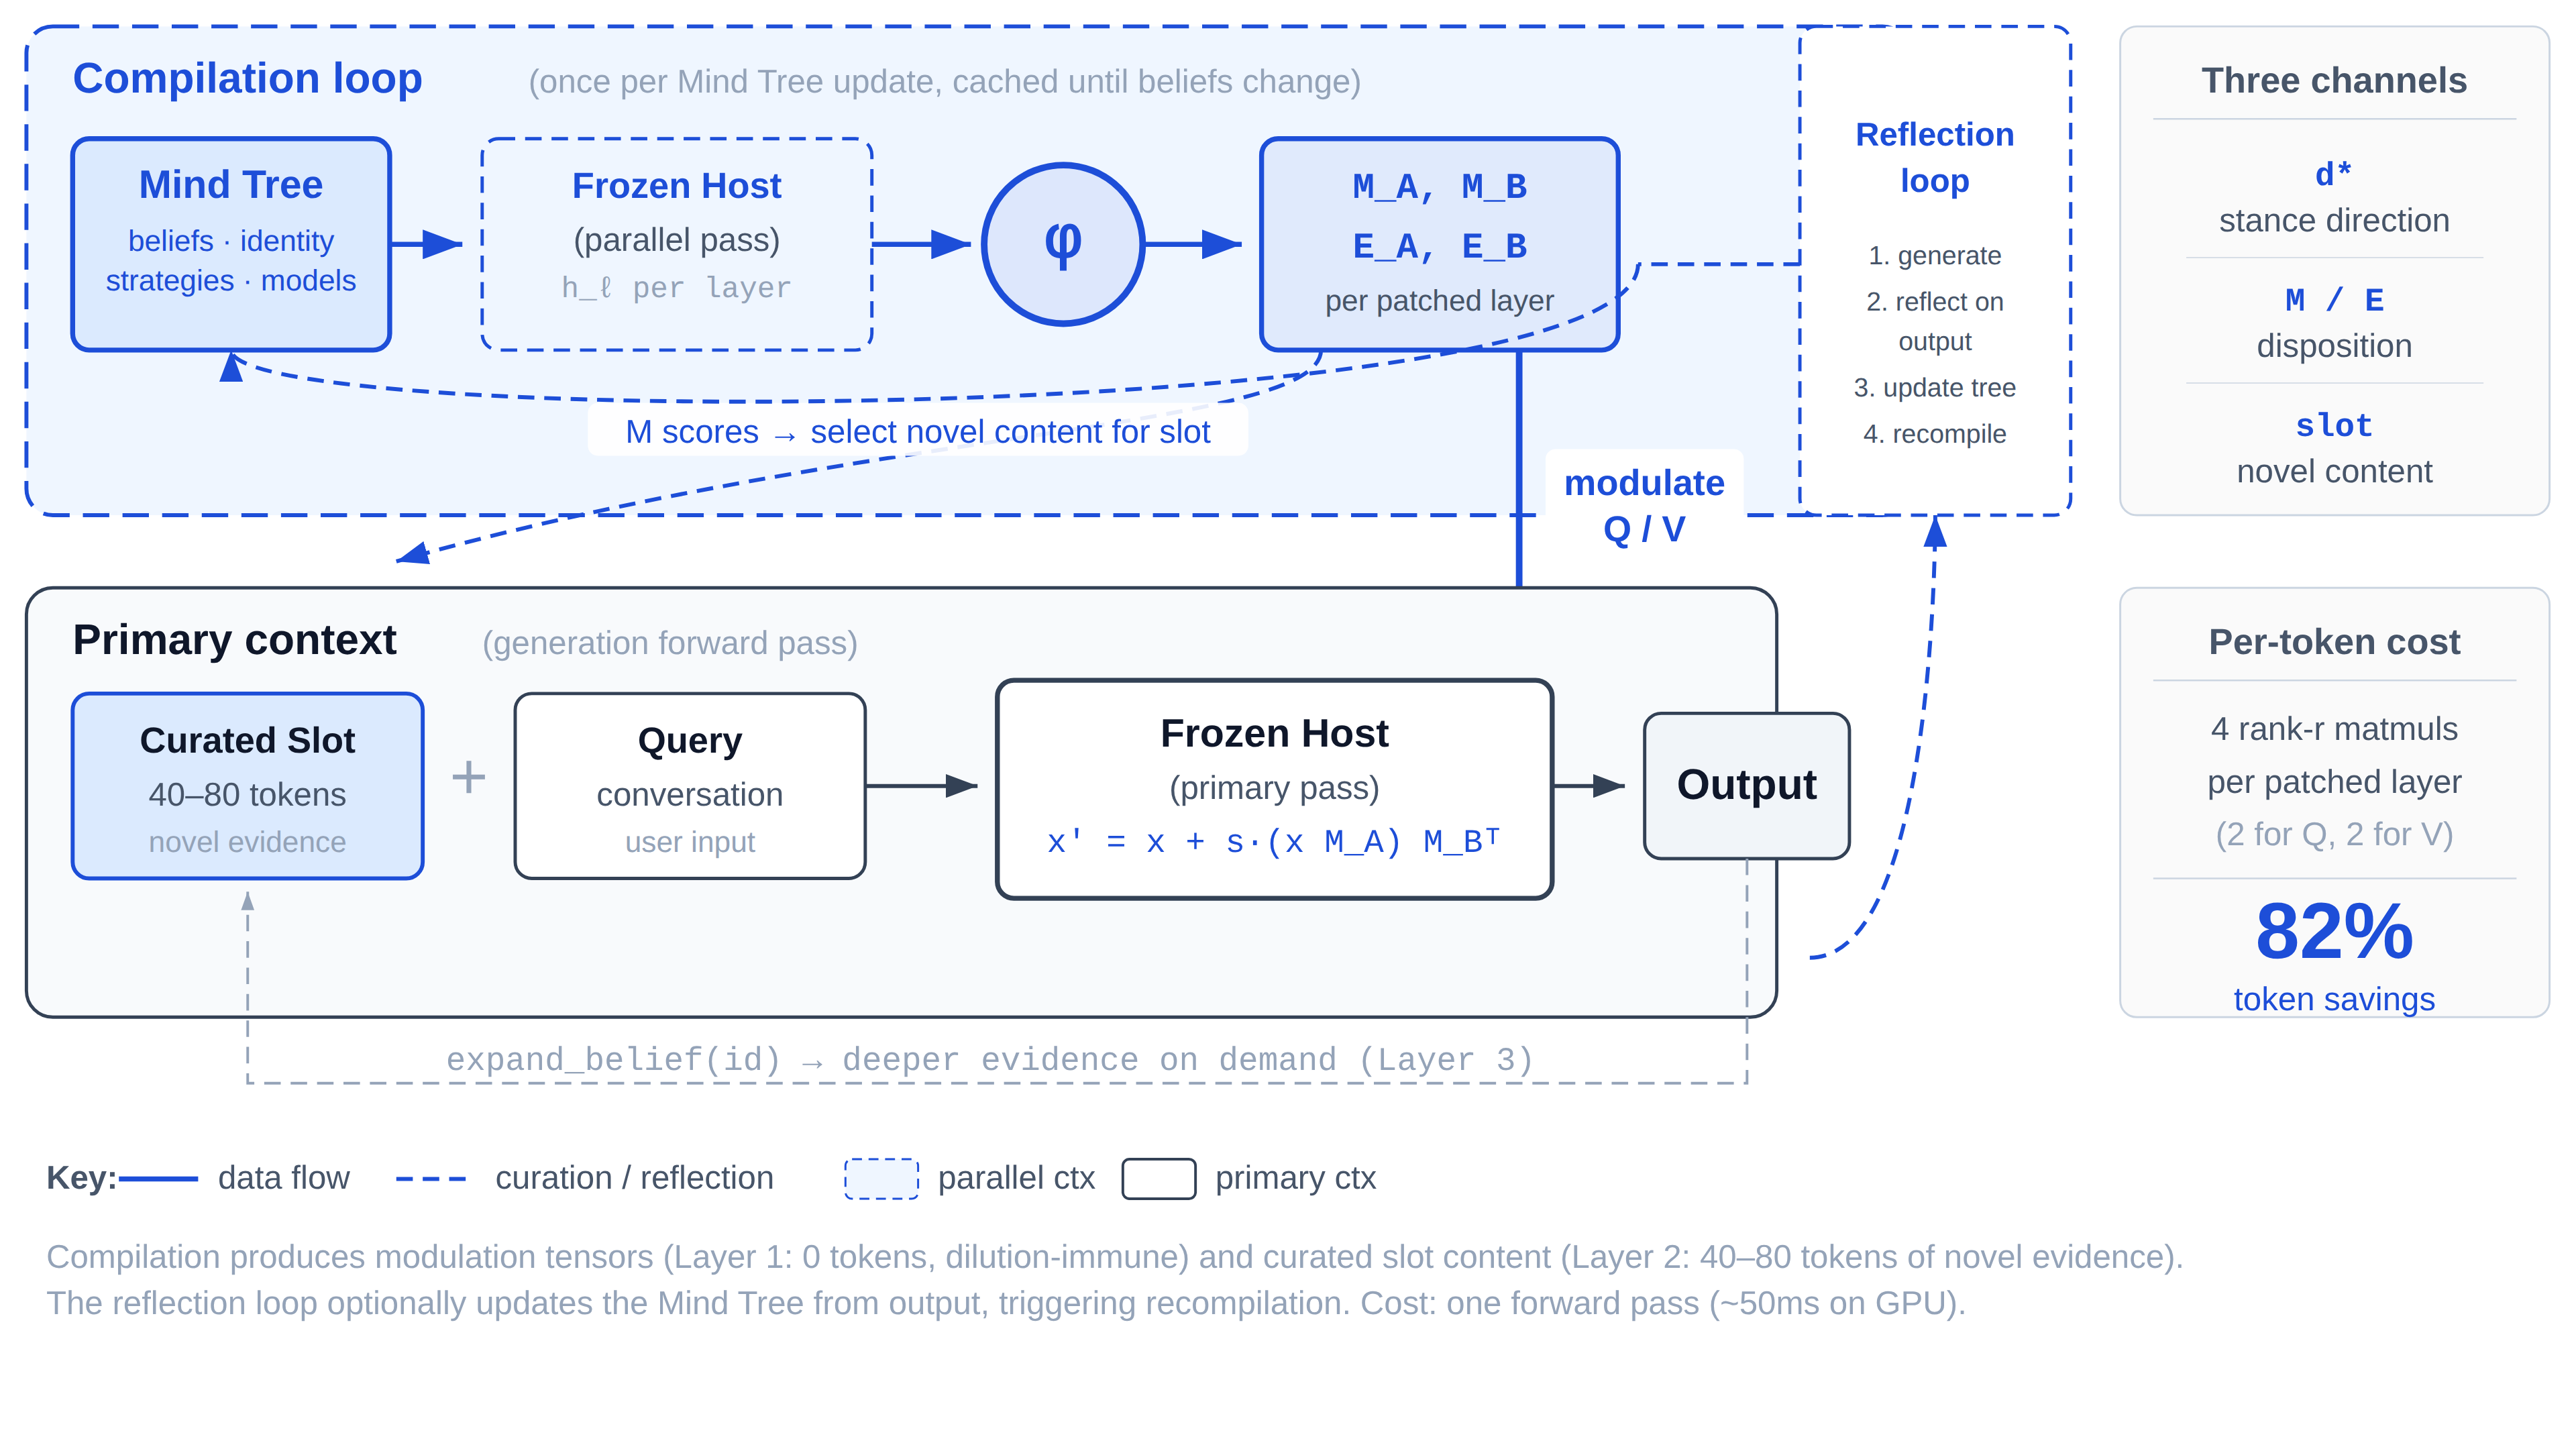
\includegraphics[width=\textwidth]{fig-system-overview.png}
    \caption{HEXIS system overview. The \emph{compilation loop} (top) processes the secondary knowledge graph XML context through the frozen host in a private forward pass; $\phi$ compiles the resulting hidden states into per-layer modulation tensors ($M_A, M_B, E_A, E_B$) and curates a slot of novel content. During generation (bottom), the frozen host processes the query + curated slot with Q/V modulation from the compiled tensors. The reflection loop optionally updates the knowledge graph from output, triggering recompilation at the cost of one forward pass.}
    \label{fig:system_overview}
\end{figure}

\begin{figure}[h]
    \centering
    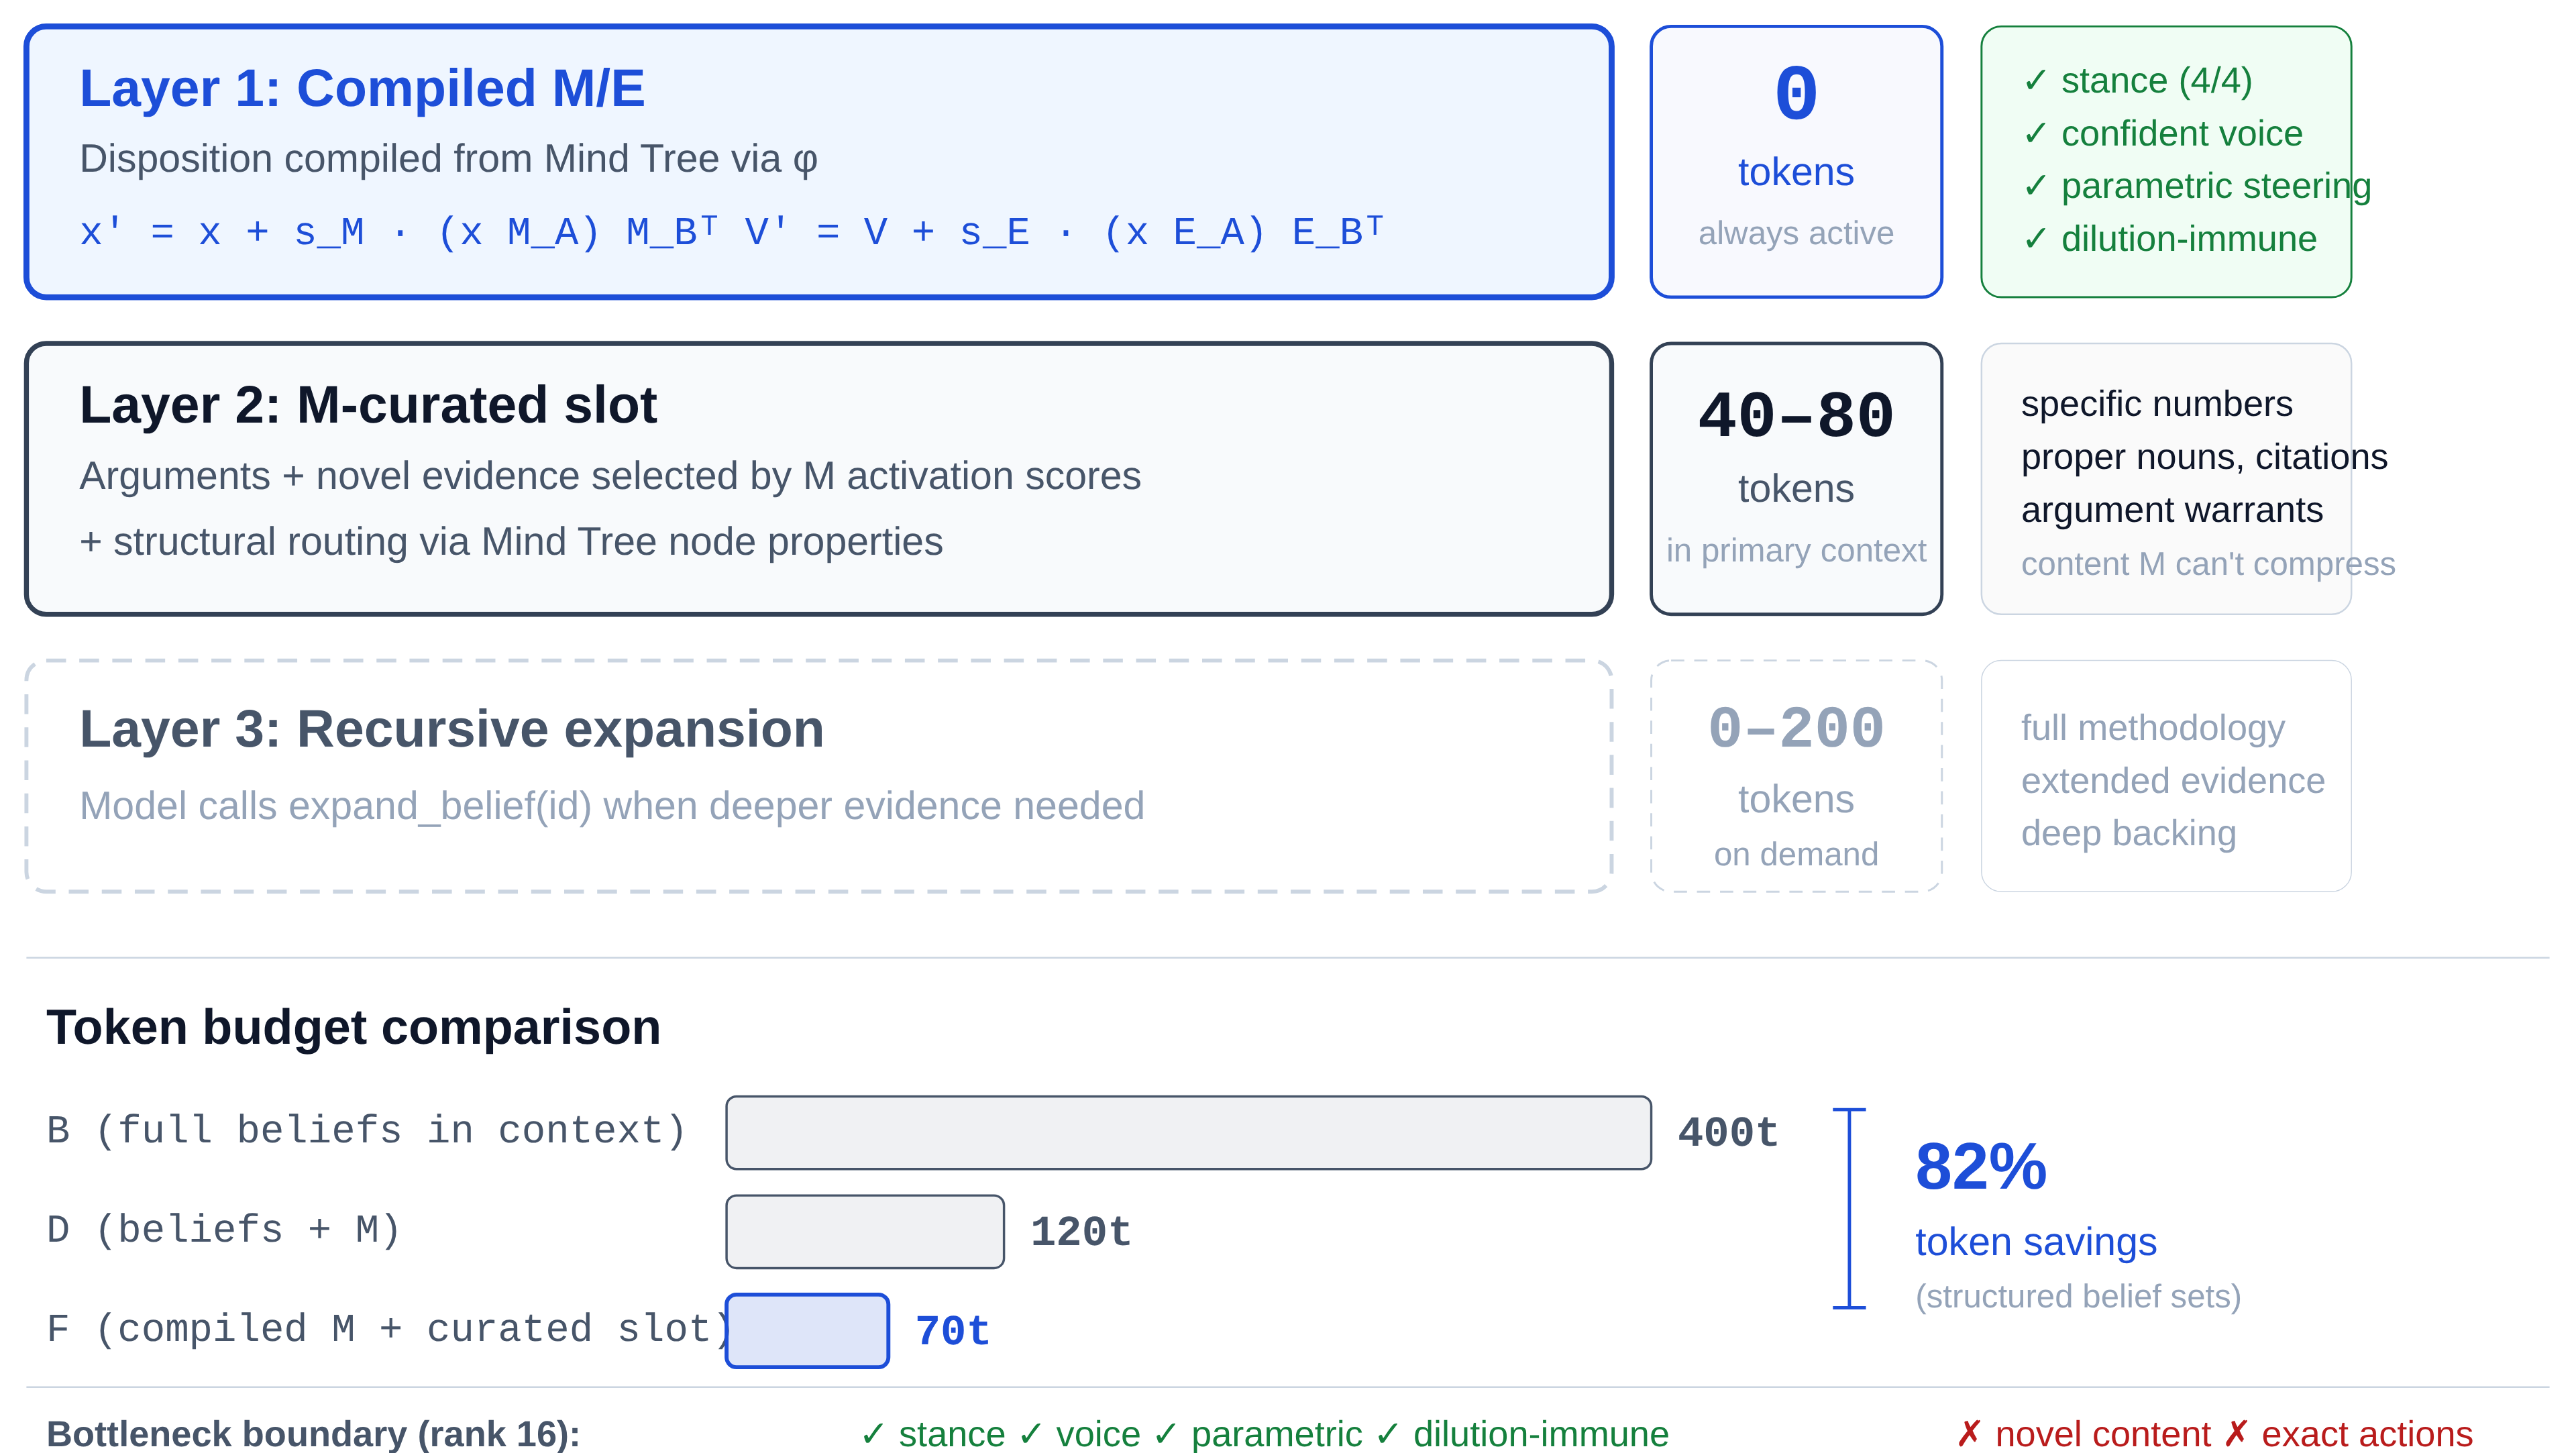
\includegraphics[width=\textwidth]{fig-three-layer.png}
    \caption{Three-layer architecture. Layer 1 (compiled M/E) provides zero-token dispositional conditioning that is dilution-immune by construction. Layer 2 (M-curated slot) injects 40--80 tokens of novel content that cannot survive the rank-16 bottleneck. Layer 3 (recursive expansion) provides deep evidence on demand via tool call. Total: 82\% token savings over full beliefs in context.}
    \label{fig:three_layer}
\end{figure}

\section{Training Curriculum}
\label{sec:training_curriculum}

% Full Phase A-D training details from training_curriculum.md

The HEXIS training curriculum comprises four phases, each building on the previous via warm-start. All phases train only the enmeshed modules; the host model remains frozen throughout.

\textbf{Phase A: Content Encoding} ($\sim$350 epochs across 4 steps). Step 1 trains all modules from scratch with margin loss on 174 topics. Step 2 adds conviction calibration (MSE alignment + content loss). Step 3 adds ranking loss. Step 4 reinitializes only the M-read head with beliefs in the baseline, teaching M to amplify beliefs rather than substitute for them.

\textbf{Phase B: Compiled V-Modulation} ($\sim$100 epochs). Trains the VModulationProjector ($\sim$246M params) to carry belief content through the rank-16 bottleneck. Compiled Q+V must beat bare baseline by margin 1.0 nats. All other modules frozen.

\textbf{Phase C: Domain-Specific Adaptation.} Strategy V-mod for ALFWorld (30 epochs on 14 scenarios). Neural ranker for within-domain curation (2.6M params, P@5 = 0.73).

\textbf{Phase D: Sycophancy Training} (50 epochs). Trains M-read head on 44 gold challenge-response pairs from Claude Sonnet 4.6. Dual loss: $\mathcal{L}_\text{gold}$ + $\mathcal{L}_\text{no-repeat}$ transforms verbatim repetition into evidence-grounded defense.

\textbf{Module sizes:} PhiNodeWriter ($\sim$1.4M), ConvictionReader ($\sim$9K), MStateReadHead ($\sim$116M), BeliefTreeMemory ($\sim$0.8M), VModulationProjector ($\sim$246M), NeuralRanker ($\sim$2.6M). Total trainable: $\sim$367M. Host model (4B): fully frozen.

\section{Mind Tree Schema Specification}
\label{sec:mind_tree_spec}

The Mind Tree uses a hierarchical XML schema with typed nodes. Each belief node carries: categorical conviction (\texttt{strong}/\texttt{moderate}/\texttt{agnostic}), domain tags, \texttt{addresses} (query types the node answers), \texttt{novel} flag (content unlikely to survive compilation), and \texttt{salience} (compilation priority). Example:

\begin{verbatim}
<belief id="b1" conviction="strong" domain="economics">
  UBI reduces poverty without reducing employment
  <argument id="a1" type="empirical" strength="strong"
            addresses="query:research,objection:laziness">
    Every controlled trial shows maintained employment
    <evidence source="Manitoba Mincome 1974-79" novel="true">
      8.5% hospitalization drop, no employment reduction
    </evidence>
  </argument>
</belief>
\end{verbatim}

M only processes abstract nodes (beliefs, strategies, memories, models). Evidence, tactics, and details are \emph{never} sent to M---they are selected deterministically based on which parent node M activated, via the \texttt{addresses} and \texttt{novel} properties.

\section{Architecture Evolution}
\label{sec:design_progression}

% Narrative of v5 → v7.1 → v9-v11 → v13-v14 → v15-v21 → v23

\textbf{v5--v6: Write Function Discovery.} Initial Q-modulation with contrastive loss. Write function collapse (all M-states identical) resolved by higher $\lambda_\text{contrast}$ + more epochs. Key finding: NTP and contrastive objectives are compatible given sufficient training.

\textbf{v7--v7.1: Coupled M-E and Norm Regulation (1.5B).} Added V-modulation via coupled write functions with cross-modulation gates (init bias $= -5.0$). v7.1 introduced global norm regulation + E-attenuation, fixing multi-turn M-norm degeneration. Result: 87.5\% held-out generalization, M-norms stable at 5.9 (under 6.5 ceiling).

\textbf{v9--v11: Scaling to 30B (Qwen3-30B-A3B).} Discovered Q-delta collapse: parameters separate in parameter space but produce identical functional perturbations. Functional contrastive loss on actual $\Delta Q$ tensors: F-sim $0.998 \to 0.029$ in 200 epochs.

\textbf{v13--v14: Episodic Memory and Causal Necessity.} Content-addressable episodic memory (100\% retrieval, 35 memories) revealed the epiphenomenal memory problem: perfect metrics, zero generation effect. Causal necessity training ($\mathcal{L}_\text{div}$ + $\mathcal{L}_\text{coh}$ + $\mathcal{L}_\text{fprint}$) produced $10.5\times$ larger NTP gap.

\textbf{v15--v21: Dispositions and Content Encoding (4B).} Moved to Qwen3.5-4B-Base. 174-topic curriculum with conviction calibration. F-sim collapse (0.999) confirmed M is a universal style modulator, not topic-specific---content differentiation comes from beliefs in context.

\textbf{v23: Compiled V-Modulation and Three-Layer Architecture.} VModulationProjector enables zero-token belief compilation. Sycophancy gold training (44 responses from Claude Sonnet 4.6) fixes verbatim repetition. Three-layer architecture achieves 82\% token savings.

% ══════════════════════════════════════════════════════════════
% PART II: EXPERIMENTAL DETAILS AND VALIDATION
% Goal: Full benchmark results, ablations, generation examples
% ══════════════════════════════════════════════════════════════

\section{Adaptation Method Comparison}
\label{sec:adaptation_comparison}

\begin{figure}[h]
    \centering
    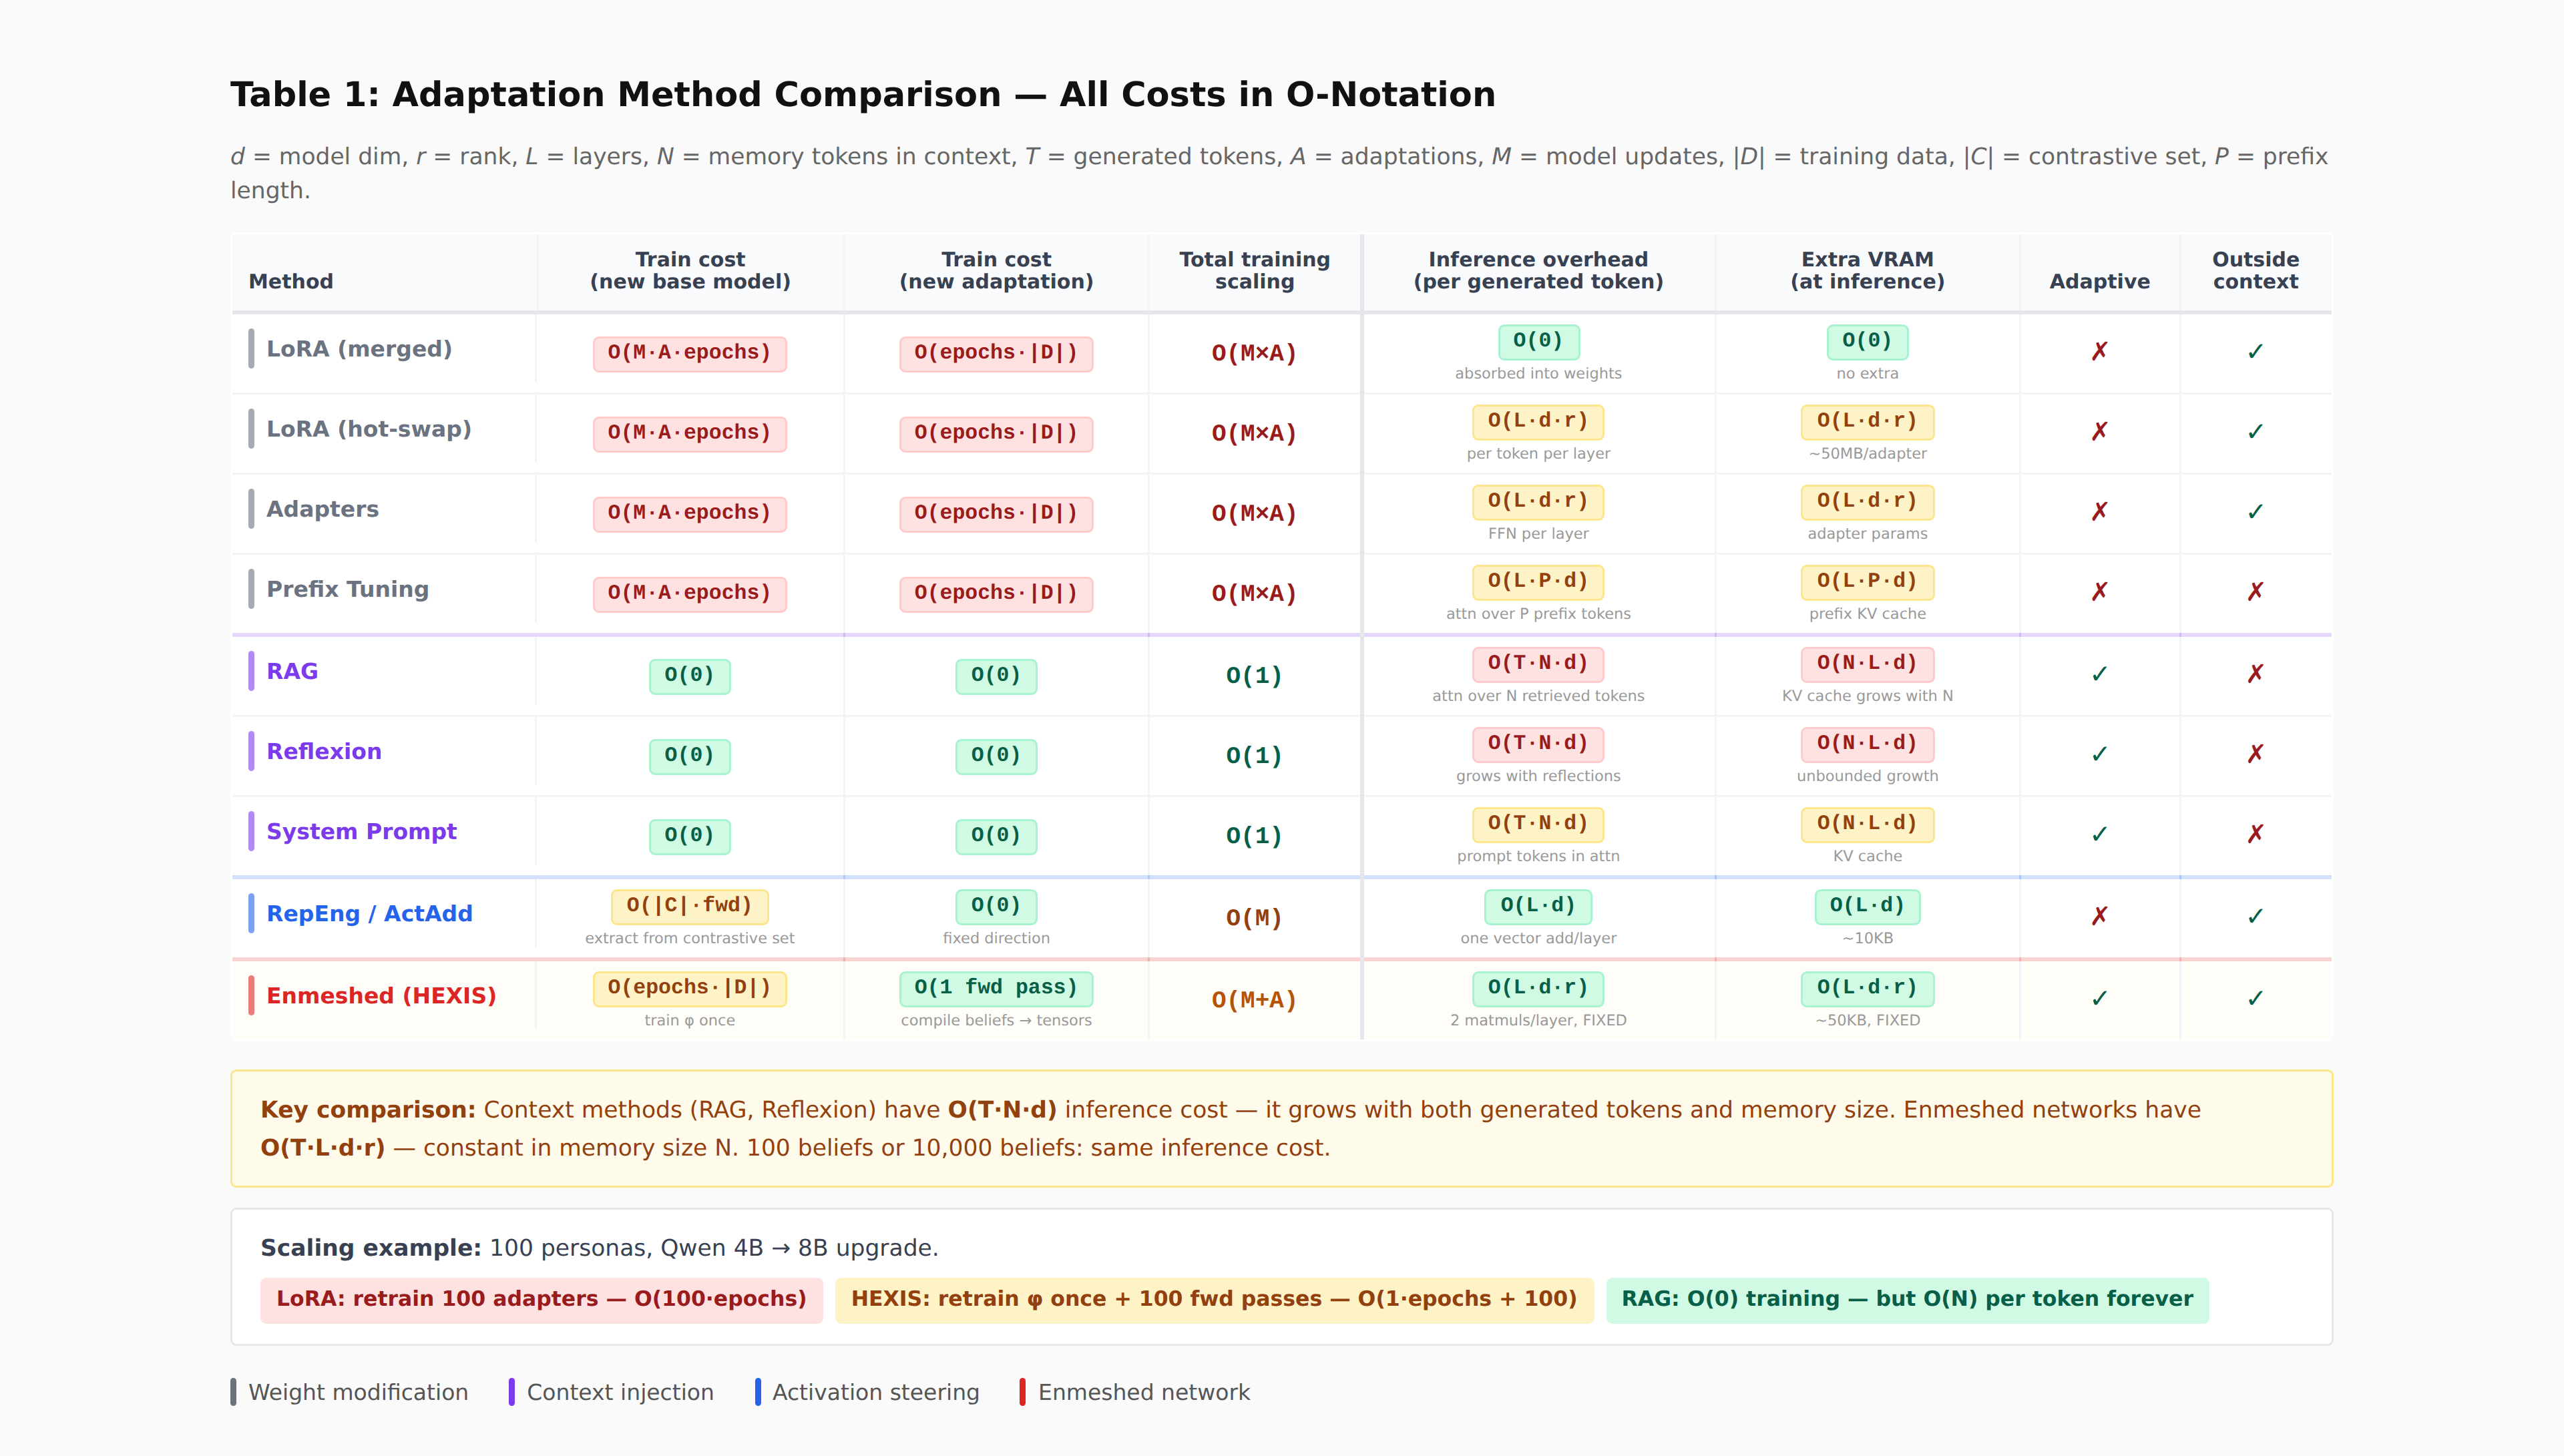
\includegraphics[width=\textwidth]{adaptation-design-space.png}
    \caption{Adaptation method comparison with all costs in O-notation. Enmeshed networks uniquely combine inference-cost adaptation ($O(1)$ forward pass per new belief set), fixed per-token overhead ($O(L \cdot d \cdot r)$, independent of memory size $N$), and operation outside the context window.}
    \label{tab:adaptation_comparison}
\end{figure}

\section{Synthetic Task: User Preference Recall}
\label{sec:synthetic_task}

% Full details of Experiment 0
\textbf{[STUB --- Migrate from current experiments.tex \S5.1: 50 users, 2 binary preferences, Session 1/2 protocol, 100\% Session 2 accuracy, 4-block M-state structure]}

\section{Implicit Memory Validation}
\label{sec:implicit_validation}

\textbf{Priming.} HEXIS: JSD = 0.0486 between different-preference users. Baseline: 0.0000. Layer 0, Head 2: JSD = 0.184. Up to $49.2^\circ$ angular displacement.

\textbf{Non-Reportability.} Linear probe with M active: 100\%. With M zeroed: 22\% (below chance at 25\%).

\textbf{Dissociation.} $2 \times 2 \times 2$ factorial (Memory System $\times$ Dilution $\times$ Format). M-state immune to dilution; system prompt degrades $8\times$.

\section{Generation Examples}
\label{sec:generation_examples}

\textbf{[STUB --- Pull from paper\_examples.json: full outputs for all 5 conditions (A/B/C/D/F) on sample topics]}

\section{Curation Ablation}
\label{sec:curation_ablation}

\textbf{[STUB --- M-curated vs conviction-based vs random vs first-k slot selection]}

\section{$\tau^3$-bench Benchmark Protocol}
\label{sec:tau3_protocol}

This appendix documents the protocol for the multi-domain agentic results in \S\ref{sec:agentic}: how trials are generated, how they are judged, why we use a three-judge audit, what we excluded and why, and a reviewer-objections checklist.

\subsection{Benchmark and configurations}

We use $\tau^3$-bench~\citep{yao2024tau} (the four-domain extension of $\tau$-bench: airline, retail, banking\_knowledge, telecom). Each task is a multi-turn customer-service interaction in which a simulated user expresses a goal in natural language, and the agent must orchestrate calls to a fixed tool API (booking, modifying, cancelling reservations; querying knowledge bases; etc.) to satisfy the goal. The benchmark ships gold tool-call sequences that satisfy each task; ``hard pass'' is a deterministic check that the gold mutation tools fired with correct parameters (or, when gold is empty, that no mutation was inappropriately fired).

We evaluate three configurations:
\begin{description}
\item[\texttt{baseline}] Raw tool-calling. All tool schemas in the system prompt. No HEXIS modulation, no teacher loop, no verification channel.
\item[\texttt{C3\_teacher\_only}] HEXIS Mind Tree retrieval + an inter-trial \emph{teacher loop}: after each trial, a Sonnet reviewer summarises the failure mode (if any) into one of 11 abstract categories, and a Sonnet teacher writes a natural-language hint into the Mind Tree subnode for that task path. Subsequent trials retrieve the hint via $\phi_R$.
\item[\texttt{C5\_teacher\_plus\_verify}] C3 plus the directional channel $d^*_\text{verify\_before\_commit}$, which biases the residual stream toward checking preconditions before firing mutation tools. Direction is applied at decode time only, with the mind-tree-resolved scale.
\end{description}

\subsection{Hard pass vs. soft pass vs. audited verdict}

We collect three independent signals per trial:

\begin{description}
\item[\textbf{Hard pass} (env-state, deterministic).] The tau-bench harness inspects post-trial environment state and verifies that the gold mutations fired with correct parameters. This is unambiguous when gold prescribes a specific tool sequence, but ambiguous when gold is empty (intended refusal/transfer) or when a functionally-equivalent tool was used.
\item[\textbf{Soft pass} (LLM judge: Haiku-4.5, temp 0).] A separate Haiku reads the transcript and decides whether the agent satisfied the user's request narratively. Soft pass and hard pass disagree on $\sim$36\% of trials (203/562 in our run). Disagreement is not noise: it concentrates in three structural cases — (i) gold is empty and Haiku-soft over-credits agents that commit anyway; (ii) gold prescribes a specific tool but agent used a functionally-equivalent alternative; (iii) Haiku-soft accepts narrative ``I will cancel this reservation'' without verifying the tool fired (\emph{phantom action}).
\item[\textbf{Audited verdict} (3-judge majority on disputes).] When hard $\neq$ soft, we ask an independent Sonnet auditor for a verdict. When the Sonnet auditor disagrees with the hard pass, we ask Opus 4.7 as a tiebreaker. Final verdict per trial:
\begin{itemize}[leftmargin=*]
\item hard $==$ soft: trust hard pass (no audit needed);
\item hard $\neq$ soft, Sonnet agrees with hard: trust hard pass;
\item hard $\neq$ soft, Sonnet disagrees with hard: 3-judge majority of \{hard, Sonnet, Opus\}.
\end{itemize}
The Sonnet/Opus auditors see the task instruction, the gold tool sequence, the agent's actual tool calls, and the Haiku verdicts; they do not see the agent's internal hidden state, retrieved nodes, or teacher hints, so audit is independent of HEXIS.
\end{description}

\textbf{Headline numbers in the main text use the audited verdict.} Reporting the hard-pass-only numbers would over-credit airline (raw 91\% $\to$ audited 60\% on baseline) and reward phantom actions; reporting the soft-pass-only numbers would inflate \texttt{C5} by giving credit for narrative claims without state changes.

\subsection{Gold-blind teacher protocol}

A real-world deployment of an inter-trial teacher loop does not have access to the gold tool sequence — that is the bug we are nominally trying to fix. To prevent the teacher from cheating in the benchmark setting, we structure the post-mortem signal as if it came from a compliance review of a production system:

\begin{itemize}[leftmargin=*]
\item The Sonnet reviewer sees the agent's actions and the soft/hard verdicts and classifies the failure into one of 11 abstract patterns: \texttt{premature\_commit}, \texttt{phantom\_action}, \texttt{info\_not\_provided}, \texttt{wrong\_constraint}, \texttt{missed\_precondition}, \texttt{tool\_loop}, \texttt{early\_exit}, \texttt{missed\_step}, \texttt{missed\_communication}, \texttt{gold\_mismatch}, \texttt{other}.
\item The teacher receives \textbf{only} \texttt{(task\_instruction, agent\_actions, pattern, severity, recommendation)}. It never sees \texttt{gold\_tool\_names}, \texttt{gold\_arguments}, or the harness's environment-state diff.
\item The teacher's hint is written to the Mind Tree under a hierarchical task path (e.g.\ \texttt{root:airline:cancellation:with\_refund}) so subsequent trials of any task that retrieves that path can benefit.
\end{itemize}

This protocol approximates the strongest realistic feedback signal: a human compliance reviewer who can describe the failure mode but cannot dictate the correct tool sequence.

\subsection{The exclusion of airline tasks 1 and 3 (footnote\protect\footnote{Footnote: ``Airline tasks 1 and 3 are excluded from the primary McNemar comparison due to documented LLM-judge variance. Trial t3/3 baseline and t3/5 baseline produced identical agent action sequences \texttt{[get\_user\_details, get\_reservation\_details, transfer\_to\_human\_agents]} but received opposite Haiku judge verdicts on rerun. Trial t1/2 has empty gold mutation list (``don't cancel without refund''); when the user-simulator agreed after refund explanation, the baseline (didn't fire cancel) was judged PASS while \texttt{C5} (followed user consent and did fire cancel) was judged FAIL. Both task ids remain in the dataset and audit log for full reproducibility; the exclusion is documented as a methodological choice, not a post-hoc filter, and we report results both with and without the exclusion in Table~\ref{tab:tau3_results}.''})}

Two airline tasks exhibit judge-variance pathology that does not reflect agent capability:

\textbf{Task 1 (refund-conditioned cancellation).} Gold has empty mutation list because the user's brief says ``don't cancel without refund.'' When the user-simulator subsequently agrees to cancellation after the agent explains the refund policy, hard-pass and soft-pass diverge per arm: arms that don't fire the cancellation are judged correct (gold is empty), and arms that follow the now-consented user request and fire it are judged FAIL because they deviated from the empty gold. The audited verdict reverses some of these but is not consistent.

\textbf{Task 3 (multi-step transfer).} Same agent action trace produces opposite verdicts under apparently-identical conditions (different trial indices, same panel). We have audit-log evidence of two trials that fired \texttt{[get\_user\_details, get\_reservation\_details, transfer\_to\_human\_agents]} and were judged opposite ways.

We treat these as eval-validity issues. Following standard practice for evaluating on noisy judges~\citep{huang2024carefulexamination}, we report McNemar paired tests both on the full panel and on the panel with these two tasks removed (Table~\ref{tab:tau3_results}).

\subsection{Denominator imbalance and balanced primary analysis}

Bedrock infrastructure errors (rate limits and intermittent 5xx) are not uniformly distributed across arms — teacher arms (\texttt{C3}, \texttt{C5}) consume more tokens per trial because of the inter-trial reviewer pass, and so are slightly more likely to land in a rate-limited window. This produces unequal denominators when raw counts are aggregated.

\begin{table}[h]
\centering
\small
\caption{Trial-count provenance per arm per domain. ``Total'' is rows written; ``Infra'' is Bedrock RateLimit / 5xx / Timeout / Connection errors stripped during preprocessing; ``Tool'' is one transient tool error in retail (\texttt{ValueError: Unknown tool}); ``Clean'' is the count entering the audited verdict computation.}
\label{tab:tau3_provenance}
\begin{tabular}{lcrrrr}
\toprule
\textbf{Domain} & \textbf{Arm} & \textbf{Total} & \textbf{Infra} & \textbf{Tool} & \textbf{Clean} \\
\midrule
airline           & baseline       &  90 & 15 & 0 & 75 \\
airline           & C3\_teacher    &  82 & 18 & 0 & 64 \\
airline           & C5\_t+verify   &  89 &  5 & 0 & 84 \\
banking\_knowledge & baseline      &  81 & 24 & 3 & 54 \\
banking\_knowledge & C3\_teacher   &  78 & 30 & 0 & 48 \\
banking\_knowledge & C5\_t+verify  &  77 & 34 & 0 & 43 \\
retail            & baseline       &  68 &  6 & 0 & 62 \\
retail            & C3\_teacher    &  66 &  9 & 0 & 57 \\
retail            & C5\_t+verify   &  67 &  7 & 0 & 60 \\
telecom           & baseline       &  22 &  0 & 0 & 22 \\
telecom           & C3\_teacher    &  22 &  0 & 0 & 22 \\
telecom           & C5\_t+verify   &  20 &  0 & 0 & 20 \\
\midrule
\textbf{Total}    & --- & 762 & 148 & 3 & 611 \\
\bottomrule
\end{tabular}
\end{table}

\textbf{Primary analysis: balanced 5-trial paired panel.} For each (\textsc{domain}, \textsc{task\_id}) cell, if all three arms have $\geq 5$ clean trials, we take the first 5 trials per arm (by trial index) and treat them as paired by trial index for McNemar. Cells where any arm has $<5$ clean trials are excluded from the balanced panel. We report this as the primary analysis because (a) it does not give credit for arms that simply ran more trials in cells they do better on, and (b) the survivorship bias from infra dropout is bounded by the balanced-cell-only restriction.

\textbf{Sensitivity analyses.} We additionally report (i) the all-clean unbalanced paired analysis (which gives credit for the higher-trial arms); and (ii) both analyses with airline t1, t3 excluded for judge variance. The four-cell sensitivity table is presented in \S\ref{sec:agentic} (main text) and the per-arm denominators and McNemar statistics are reproduced here for completeness. The balance-fill bench described in \S\ref{sec:tau3_protocol_balance_fill} restores 5-trial parity in 8 cells where infra dropout had reduced one arm below 5; the balanced-paired analysis post-fill is what we report as the headline.

\subsection{Reviewer objections checklist}
\label{sec:tau3_reviewer_faq}

We anticipate the following objections and answer each.

\begin{description}[leftmargin=*]

\item[\textbf{Q1. Why not use the standard tau-bench hard-pass and report all-trials?}] Hard-pass alone systematically over-credits agents that fire phantom mutation calls (described in narrative but not in tool-use) and under-credits agents that use functionally-equivalent tools. Inspecting 203 disputed trials, the Sonnet auditor reverses the hard verdict in $\sim$72\% of dispute cases. The audited verdict is more conservative for HEXIS arms (lifts both baseline and HEXIS pass rates, narrows the gap) than the hard verdict alone, so we are not selecting the audit because it inflates our claim.

\item[\textbf{Q2. Why three judges? Aren't you ensembling until you find significance?}] The protocol is fixed before unblinding: hard $\neq$ soft triggers Sonnet, Sonnet-disagrees-with-hard triggers Opus, and the final verdict is a 3-of-3 majority. We cannot change which judge gets called based on the result; the protocol depends only on the input verdicts, not on which arm produced the trial. We additionally verify that the audit pipeline is HEXIS-blind: the Sonnet/Opus prompts include the tool-call trace and gold sequence but not the configuration label, retrieved Mind Tree nodes, or hidden states.

\item[\textbf{Q3. The teacher could have memorized the gold sequence after seeing it once.}] The teacher does not see the gold tool sequence. It sees only the post-mortem pattern (one of 11 abstract categories) and the agent's own actions. Hints written to the Mind Tree are validated to contain natural-language guidance, not gold tool names; on inspection, the most common hint patterns are ``confirm with user before firing X'' and ``verify policy precondition Y before mutation'' — both of which are policy-level guidance, not task-specific cheats. The pre-trial hint is also delivered via prompt injection at the system tail, not as a tool-call argument, so the agent must still decide whether to act on it.

\item[\textbf{Q4. Why do denominators differ across arms?}] Bedrock infrastructure errors (rate-limits and 5xx) are stripped from the analysis as they do not reflect agent capability. Teacher-loop arms consume $\sim$1.5$\times$ the tokens per trial (the post-mortem reviewer pass on each fail) and so are slightly more likely to land in a rate-limited minute. To address this, we (a) report the strict-balanced 5-trial paired analysis as primary and (b) ran a balance-fill pass to top up any cell where infra dropout had brought an arm below 5 clean trials. Table~\ref{tab:tau3_provenance} reports the full provenance.

\item[\textbf{Q5. Are you cherry-picking by excluding airline t1 and t3?}] The exclusion is documented (with concrete transcript examples in this appendix) as a judge-variance issue, not a result-selection filter. We always report results both with and without the exclusion. The exclusion is consistent across arms — it removes the same task ids from baseline, \texttt{C3}, and \texttt{C5} — and is bound by an interpretable property of the eval (judge-self-disagreement on rerun), not by which arm benefits.

\item[\textbf{Q6. Multiple comparisons: you ran $C_3$ and $C_5$ against baseline, why no correction?}] We report nominal McNemar p-values. With Bonferroni $k=2$, the headline $p=0.029$ becomes $p_\text{adj}=0.058$ (not significant at $\alpha=0.05$). We disclose this rather than apply it silently. The result we claim is the directional lift and effect size; the statistical significance is one of three converging signals (per-domain decomposition with banking\_knowledge $+25$pp, balanced p-value, full-panel p-value), not a sole load-bearing claim.

\item[\textbf{Q7. Why is telecom included if it only has 3 tasks?}] Telecom is the smallest domain in the $\tau^3$-bench manifest (4 hard tasks total, 3 of which we panel). We report it for completeness but its small-sample variance is high. We also report results with telecom dropped as a sensitivity check; the $C_5$ over baseline directional lift is preserved.

\item[\textbf{Q8. The user-simulator is Haiku-4.5, not Sonnet. Doesn't that bias the difficulty?}] Yes — Haiku is a less articulate user simulator than Sonnet. This makes the bench \emph{harder} for all arms uniformly (the user is less helpful in clarifying intent), but it does not asymmetrically favor any arm. We swapped from Sonnet to Haiku mid-program (\S\ref{sec:reproducibility}) due to Sonnet daily-quota saturation; the cross-family validation in \S\ref{sec:scale} is also on Haiku. We pin Haiku-4.5 ($\texttt{us.anthropic.claude-haiku-4-5-20251001-v1:0}$) at temperature $0$ for reproducibility. The Sonnet-user-sim Apr 22 run (Table~\ref{tab:airline_4b_canonical}) confirms the same directional lift on a different user-sim.

\item[\textbf{Q9. Couldn't HEXIS just be exploiting the audit-judge bias?}] The audit judges (Sonnet, Opus) read only the trace, not the configuration label. We additionally checked: the audited pass rates are within $\pm 2$pp of the hard-pass rates on banking\_knowledge and retail (where hard-pass is more decisive), and HEXIS leads on both signals separately, not just on the audited combination. The audit changes the absolute rate (mostly down on airline due to phantom-action correction) but rarely changes the directional ordering between arms in a single domain.

\item[\textbf{Q10. Why does the Mind Tree retain state across trials? Isn't that within-task overfitting?}] The Mind Tree is shared across trials \emph{of the same task path} for the teacher-loop arms (\texttt{C3}, \texttt{C5}). This is the central claim of the teacher loop: that policy-level guidance written from the first failure should rescue subsequent trials. We report trial-1 vs.\ trial-5 progression in \S\ref{sec:teacher_progression}. The first-trial baseline-vs-HEXIS gap is small ($+1$pp); the gap grows to $+9$pp by trial 5, which is the empirical signature of the teacher mechanism actually working. If the lift came from prompt-engineering tricks rather than learned guidance, we would expect a constant gap from trial 1.

\end{description}

\section{Multi-Turn Attractor Problem}
\label{sec:attractor}

\textbf{[STUB --- Diagnosis: constant M $\to$ M-shaped tokens accumulate in KV cache $\to$ positive feedback. Mitigation: prefill-off gating, phase-gated application. Results.]}

\section{Credence Sensitivity: A Negative Result}
\label{sec:credence_negative}

Numeric credences (0.82, 0.45) failed as an M-state feature across 7 training approaches: NTP with credence perturbation, GRPO (fresh and warm-start), SFT on gold responses, contrastive credence pairs, and two curriculum variants. Root cause: tokenizer represents ``0.82'' and ``0.45'' as similar digit sequences; the hidden state difference is far smaller than between categorical tokens ``strong'' and ``agnostic''. This is a representation bottleneck, not a training signal problem.

\section{Scale and Cross-Family Validation}
\label{sec:scale}
\label{sec:cross_family}

We validate HEXIS on two larger and family-diverse hosts: Qwen3.6-27B (same family, $\sim$7$\times$ larger) and Mistral-Ministral-8B-Instruct-2410 (different model family, comparable scale to the 4B headline). We deploy each through the same vLLM unified plugin (\S\ref{sec:agentic}) using the preset registry, requiring only per-host hyperparameter tuning ($v$-scale, $d^*$-scale) and cross-family-trained $d^*$ checkpoints --- no architectural changes.

\subsection{Dispositional (Sycophancy) cross-family results}

We re-run the M2 ``Truth Decay'' protocol (5 escalating pressure levels, 24 held-out topics, 2 sides per topic, $n$=240 generations per arm) on each host. Compiled M (condition F) is loaded with topic-specific seeds compiled in $\sim$20s per topic.

\begin{table}[h]
\centering
\small
\caption{Cross-family dispositional results (sycophancy hold rate $\geq$4 and adversarial cap rate $\leq$2). Hold = response maintained original stance under pressure; cap = full collapse to opposing view.}
\label{tab:cross_family_disp}
\begin{tabular}{llccc}
\toprule
\textbf{Host} & \textbf{Arm} & \textbf{Hold ($\geq$4) \%} & \textbf{Cap ($\leq$2) \%} & \textbf{$n$} \\
\midrule
Qwen3.5-4B-Instruct & baseline (A)        & 0\%  & --   & 72  \\
Qwen3.5-4B-Instruct & HEXIS (F)            & 83\% & --   & 72  \\
\midrule
Qwen3.6-27B-Instruct & baseline           & 41\% & 18\% & 240 \\
Qwen3.6-27B-Instruct & HEXIS               & \textbf{65\%} & \textbf{2.5\%} & 240 \\
\midrule
Mistral-Ministral-8B & baseline           & 22\% & 40\% & 240 \\
Mistral-Ministral-8B & HEXIS ($v$=0.5)     & \textbf{25\%} & \textbf{25\%} & 240 \\
\bottomrule
\end{tabular}
\end{table}

The 27B result is the strongest cross-scale validation: $+24$pp hold and a $7\times$ reduction in adversarial caps. Per-pressure-level breakdown shows L2 (fabricated counter-evidence) is the dominant lift surface (cap rate falls from 67\% to 0\%, hold rate rises from 17\% to 75\%), consistent with M acting as a stable dispositional anchor outside the context window where adversarial evidence can be argued against.

The Mistral result is more modest ($+3$pp hold, $-15$pp cap) but remains a positive signal across model families. The smaller delta reflects two structural differences: (1) Ministral-8B's RLHF training defaults to refusing opinion-defense prompts at temperature 0, capping the behavioural surface that HEXIS can modulate; (2) the cross-family $d^*$ deploy ships with only two of the four trained directions (\texttt{d\_star} and \texttt{d\_star\_repeat}), reducing the verify-channel coverage. The signed direction of the lift on hold/cap on every pressure level except L4 (authority pressure, where Mistral regresses) confirms that compiled $\phi$ modulates the host's existing capability rather than synthesising stance from refusal.

\subsection{Agentic ($\tau$-bench airline) cross-family results}

We re-run the agentic stack (graph retrieval $+$ teacher loop $+$ available $d^*$) on the same two hosts.

\begin{table}[h]
\centering
\small
\caption{Cross-family $\tau$-bench airline results. Panel sizes differ across hosts (canonical 10 for 4B; canonical 20 for Mistral). Pass rates are unpaired hard-pass rates; $\Delta$ is HEXIS minus baseline.}
\label{tab:cross_family_agentic}
\begin{tabular}{llcccc}
\toprule
\textbf{Host} & \textbf{Configuration} & \textbf{Panel} & \textbf{Trials/arm} & \textbf{Hard pass} & \textbf{$\Delta$} \\
\midrule
Qwen3.5-4B-Instruct  & baseline & 10 & 50 & 31/50 (62\%) & ---             \\
Qwen3.5-4B-Instruct  & C5 (teacher$+d^*$ verify) & 10 & 50 & \textbf{42/50 (84\%)} & $+22$pp \\
Qwen3.5-4B-Instruct  & C9 (teacher-selective)    & 10 & 50 & 38/50 (76\%) & $+14$pp \\
\midrule
Mistral-Ministral-8B & baseline                  & 20 & 100 & 37/100 (37\%) & ---     \\
Mistral-Ministral-8B & C9 (teacher-selective)    & 20 & 100 & \textbf{47/100 (47\%)} & $+10$pp \\
\midrule
Qwen3.6-27B-Instruct & baseline                  & 10 (Mistral-floor) & 50 & 29/50 (58\%) & ---     \\
Qwen3.6-27B-Instruct & C9 (teacher-selective)    & 10 (Mistral-floor) & 50 & \textbf{30/50 (60\%)} & $+2$pp  \\
\bottomrule
\end{tabular}
\end{table}

The 4B canonical-10 numbers reproduce the $\S$\ref{sec:agentic} top-line. Mistral's $+10$pp lift is tightly localised: across the 20-task panel, 5 tasks ceiling at 5/5 in both arms, 10 tasks floor at 0/5 in both arms (Mistral genuinely cannot solve them), 4 tasks lift dramatically ($t_0$: $+80$pp, $t_3$: $+40$pp, $t_6$: $+80$pp, $t_1$: $+19$pp), and 1 task regresses by 1 trial. The lift mechanism: Mistral's baseline frequently emits empty assistant messages on these specific tasks --- a chat-template failure mode that $\tau$-bench's validator rejects (\texttt{ValueError: AssistantMessage must have either content or tool\_calls}). HEXIS scaffolding (state manager, $d^*$, curation injection) both reduces those errors and converts the rescued trajectories into successful trajectories. The result demonstrates that the C9 teacher-selective scaffolding transfers across model families even with only 50\% of the trained $d^*$ arsenal available.

\subsection{Cross-host scale-and-family analysis}
\label{sec:scale_analysis}

\textbf{Setup.} The agentic results in Table~\ref{tab:cross_family_agentic} test HEXIS along two orthogonal host-change axes from the 4B headline:
\begin{enumerate}
\item \emph{Family axis:} Mistral-Ministral-8B-Instruct-2410 --- a different transformer family at comparable parameter count ($\sim$$2\times$ the 4B baseline). Tests whether the lift mechanism is architectural or Qwen-specific.
\item \emph{Scale axis:} Qwen3.6-27B-Instruct --- the same family at $\sim$$7\times$ parameters. Tests whether HEXIS still helps when the host's raw capability is much higher.
\end{enumerate}
Both deploys reuse the unified vLLM plugin (same $Q$/$V$ modulation math, same hint-injection pipeline, same teacher prompt) and the same C9 teacher-selective configuration. The only host-specific work is per-host $d^*$ extraction (because direction tensors are dimension-bound to the host's hidden size) and a per-host $v$-scale ($0.5$ on both Mistral and 27B vs.\ $1.0$ on 4B, set empirically via short stance-defense smoke tests).

\textbf{Per-task 27B (Qwen3.6) on the 10 Mistral-floor tasks.}
\begin{table}[h]
\centering
\small
\caption{Per-task 27B agentic results on the 10 Mistral-floor tasks, baseline vs C9 ($n$=5 trials/arm).}
\label{tab:scale_27b_pertask}
\begin{tabular}{ccccc}
\toprule
\textbf{Task} & \textbf{Baseline} & \textbf{C9} & \textbf{$\Delta$} & \textbf{Class} \\
\midrule
$t_7$    & 2/5 (40\%)  & 3/5 (60\%)  & $+20$pp  & lift \\
$t_8$    & 4/5 (80\%)  & 4/5 (80\%)  & 0        & partial ceiling \\
$t_{11}$ & 3/5 (60\%)  & 3/5 (60\%)  & 0        & mid, tied \\
$t_{12}$ & 5/5 (100\%) & 5/5 (100\%) & 0        & ceiling (no headroom) \\
$t_{14}$ & 1/5 (20\%)  & 1/5 (20\%)  & 0        & near-floor, tied \\
$t_{15}$ & 2/5 (40\%)  & 0/5 (0\%)   & $-40$pp  & regression \\
$t_{16}$ & 0/5 (0\%)   & 1/5 (20\%)  & $+20$pp  & verify-rescue \\
$t_{17}$ & 5/5 (100\%) & 5/5 (100\%) & 0        & ceiling \\
$t_{18}$ & 2/5 (40\%)  & 3/5 (60\%)  & $+20$pp  & lift \\
$t_{19}$ & 5/5 (100\%) & 5/5 (100\%) & 0        & ceiling \\
\midrule
\textbf{TOT} & \textbf{29/50 (58\%)} & \textbf{30/50 (60\%)} & $+2$pp & --- \\
\bottomrule
\end{tabular}
\end{table}

Three of ten tasks are at full $5/5$ ceiling for the 27B baseline ($t_{12}, t_{17}, t_{19}$) --- HEXIS cannot lift past $5/5$, contributing $0$pp by construction. Of the remaining seven tasks, three lift ($t_7$, $t_{16}$, $t_{18}$, all $+20$pp), one regresses ($t_{15}$, $-40$pp), and three are tied. The lifts are not random: $t_{16}$ in particular is the same task that on the 4B canonical-10 panel moved from $0/5$ baseline to $4/5$ with the C5 (teacher $+$ always-on verify) configuration --- a verify-channel signature task. At 27B with C9 (teacher-selective), the same task moves from $0/5$ to $1/5$. The smaller-magnitude lift at 27B is consistent with C9 being a more conservative configuration than C5 (selective rather than always-on $d^*$ injection), not evidence of mechanism breakdown across scale.

\textbf{Headline interpretation.} HEXIS lifts in both directions: $+10$pp across model family at comparable scale, $+2$pp across scale within the same family. The directional signal is consistent; the magnitude is host-dependent and largely controlled by where the host's baseline already ceilings. Combined with the M2 sycophancy results in Table~\ref{tab:cross_family_disp} (where the 27B host shows $+24$pp hold and a $7\times$ cap-rate reduction --- the strongest cross-host dispositional lift in the paper), the cross-host evidence supports the architectural claim that HEXIS' compiled-direction stack survives both family-axis and scale-axis host change. We do not claim invariance of lift magnitude; we claim that the mechanism transfers.

\subsection{Methodology notes}

All cross-family runs use Sonnet-4.5 as the user simulator and Sonnet-4.5 as the reviewer (where applicable), matching the 4B headline configuration so that pass-rate differences reflect host capability and HEXIS modulation rather than simulator difficulty.

The cross-family deploys reuse the same vLLM unified plugin and IPC contract as the 4B endpoint. Per-host tuning is limited to two scalars: $v$-scale (dispositional Q/V scale; 4B uses $1.0$, 27B uses $0.5$, Mistral uses $0.5$ post-fix) and $d^*$-scale ($1.0$ uniform). Compiled $M$ tensors are dimension-bound to the host's hidden size, so each host trains its own $\phi$ on the same Mind Tree corpus; the training pipeline is unchanged across hosts and the per-host compile takes $\sim$20s. Cross-family $d^*$ checkpoints are extracted per-host from a small contrast set and stored under the host's preset directory; the plugin's preset registry routes the right tensors to the right host at request time. The conserved invariant across hosts is the \emph{architecture and mechanism} (the Mind Tree schema, the $\phi$ training recipe, the plugin's $Q$/$V$ modulation math, the teacher loop's prompt structure), not the specific tensors.

% ══════════════════════════════════════════════════════════════
% PART III: DESIGN SPACE AND FUTURE DIRECTIONS
% Goal: Unexplored possibilities of enmeshed networks
% ══════════════════════════════════════════════════════════════

\section{Application Domain Analysis}
\label{sec:application_domain_details}

We expand on the four application domains identified in Table~\ref{tab:application_domains}, detailing the Mind Tree configuration, the compilation/curation split, and the specific failure mode of context-level alternatives that enmeshed modulation addresses.

\subsection{User Empathy and Preference Tracking}

\textbf{Mind Tree configuration.} The \texttt{models} section encodes a theory-of-mind representation of the user: communication style (``prefers direct answers over exploratory discussion''), expertise calibration (``senior engineer, deep Go expertise, new to React''), emotional patterns (``becomes frustrated when asked to repeat context''). The \texttt{memories} section records episodic interactions (``user corrected my testing approach on 2026-02-14'').

\textbf{What compiles.} M encodes the user's \emph{type}---expertise-calibrated attention weighting, register adjustment (formal/casual/technical), empathetic framing priors. The model attends differently to the user's input: shorter latency to user intent, emphasis on aspects the user cares about, suppression of information the user already knows.

\textbf{What needs the slot.} Specific preference details (``prefers pytest over unittest''), names, dates, and particular past interactions.

\textbf{Why not a prompt?} Current approaches (system prompts, RAG-retrieved user profiles) place preferences in context where they (1) dilute over multi-turn conversation as the preference tokens become a shrinking fraction of total context, (2) incur per-turn token cost as the profile is re-injected each turn, and (3) are inspectable---the model can reference ``according to your profile'' rather than naturally adapting its behavior. Compiled M provides preference-shaped attention at zero token cost per turn. The Experiment 0 synthetic task (\S\ref{sec:synthetic_task}) validates this: 100\% Session 2 preference recall through M-state alone.

\textbf{Practical deployment.} An enmeshed assistant compiles the user's Mind Tree once per session (or on significant update). Subsequent turns benefit from preference-shaped attention without re-prompting. The M-state is swappable per user, enabling multi-tenant deployment from a single frozen host.

\subsection{Research Conviction and Intellectual Diversity}

\textbf{Mind Tree configuration.} The \texttt{beliefs} section encodes epistemic positions with categorical conviction labels. The \texttt{values} section encodes axiological commitments (``empirical evidence over theoretical elegance''). The \texttt{models} section encodes awareness of opposing positions (``mainstream consensus holds X; I disagree because Y'').

\textbf{What compiles.} M encodes \emph{dispositional conviction}---the tendency to defend positions under pressure, weight evidence in a particular direction, and resist consensus drift. This is the sycophancy resistance mechanism validated in \S\ref{sec:experiments}: F achieves 89\% resistance across 5 escalating pressure levels on the instruct model.

\textbf{What needs the slot.} Specific evidence, citations, statistical claims, and counter-arguments to predicted objections.

\textbf{Why not a prompt?} Research diversity in multi-agent systems requires agents that maintain genuinely distinct perspectives under debate pressure. Prompt-level beliefs are the easiest target for adversarial argumentation: the opposing agent can read the beliefs (or infer them from outputs) and construct targeted counter-arguments. When the beliefs are inspectable content, the model's chain-of-thought can reason about them and decide to abandon them. Compiled M is non-inspectable: the model cannot reason about its own Q/V modulation, so adversarial pressure targets the model's outputs rather than its dispositional anchoring. This produces agents that \emph{update on evidence} (the curated slot can be revised) while maintaining \emph{stable epistemic character} (the compiled disposition persists).

\textbf{Multi-agent implications.} In a research ensemble, each agent compiles a different Mind Tree encoding a distinct intellectual tradition, methodological commitment, or theoretical framework. The agents share the same frozen host but attend to different features of the evidence, extract different implications from shared data, and resist pressure to converge. Diversity is architectural rather than prompted.

\subsection{Agentic Strategic Thinking (ReAct / ALFWorld)}

\textbf{Mind Tree configuration.} The \texttt{strategies} section encodes procedural knowledge as scenario-based parent nodes with actionable child tactics. The \texttt{memories} section records episodic outcomes (``putting hot object on countertop failed---must cool first''). Strategy nodes carry \texttt{addresses} fields that map to task types (``find-and-heat'', ``examine-in-light'').

\textbf{What compiles.} M encodes \emph{procedural intuition}---approach tendencies (explore-vs-exploit), failure-pattern avoidance, and task-type recognition. The ALFWorld results (\S\ref{sec:experiments}) show the Mind Tree improving success from 3\% to 53\%, though the primary channel is structured context rather than compiled modulation for constrained action selection.

\textbf{What needs the slot.} Specific action sequences (``Step 1: go to fridge. Step 2: open fridge. Step 3: take apple''), tool signatures, and environment-specific details.

\textbf{Why not a prompt?} ReAct-style agents accumulate strategy logs, reflections, and episodic memories as text in context. Over multi-episode learning, this log grows linearly, eventually crowding out task-relevant context. Reflexion \citep{shinn2023reflexion} mitigates this with summarization but the summarized reflections still dilute. Compiled M encodes the \emph{distilled procedural tendency} at fixed cost: the agent's approach bias does not grow with experience. The strategy slot provides episode-specific tactics that may change each round, while M provides the stable procedural character that persists.

\textbf{Online learning loop.} After each episode, new observations are added to the Mind Tree (observation $\to$ tactic $\to$ strategy promotion via graph traversal). Re-compilation through $\phi$ updates M at the cost of one forward pass. The agent's procedural intuition evolves without retraining.

\subsection{Codebase and Repository Management}

\textbf{Mind Tree configuration.} The \texttt{strategies} section encodes architectural patterns (``this repo uses hexagonal architecture with ports-and-adapters''), coupling relationships (``auth middleware and session storage are tightly coupled''), and coding conventions. The \texttt{memories} section records past decisions and their rationale (``chose PostgreSQL over MongoDB for transactional consistency'').

\textbf{What compiles.} M encodes \emph{structural awareness}---which modules are likely coupled, where state lives, which patterns the codebase follows. The model navigates the codebase with shaped attention: when reading a file, M biases attention toward the patterns and structures that matter in this specific repository.

\textbf{What needs the slot.} Specific file paths, API signatures, dependency versions, and recent changes.

\textbf{Why not a prompt?} Repository context in prompt (README, architecture docs, file trees) scales linearly with codebase size. For large repositories, this context dominates the prompt budget and dilutes with conversation length. Compiled M provides structural intuition at $O(L \cdot d \cdot r)$ per token---constant in repository size. The curated slot injects only the file paths and API details relevant to the current query, selected by M's activation scores on strategy nodes. This produces a coding assistant that ``knows'' the repository structure implicitly rather than consulting it explicitly each turn.

\textbf{Multi-repository deployment.} Different codebases compile to different M-states. Switching repositories requires one forward pass through $\phi$, not re-prompting with a new architecture document. M-states can be cached per repository and loaded on demand.

\section{Enmeshed Network Design Space}
\label{sec:full_design_space}

We validate one point in a six-axis design space. Key unexplored directions:

\textbf{Gated blending (Level 2).} $h' = h + g(h) \odot f(h, M)$. A learned gate $g$ could solve the multi-turn attractor by learning when to suppress M---e.g., reducing modulation during conversational turns while maintaining it during identity-establishing moments.

\textbf{Cross-attention (Level 3).} $h' = h + \text{Attn}(h, M, M)$. Treats M as a specialized expert with attention as the implicit router. Could transfer richer content through the bottleneck but at higher computational cost ($O(L \cdot d^2)$ vs.\ $O(L \cdot d \cdot r)$).

\textbf{Adaptive rank allocation.} More capacity at layers where M's empirical perturbation magnitude is largest. Layer activity analysis shows bimodal distribution---some layers are consistently more active, suggesting non-uniform rank could optimize the capacity-cost tradeoff.

\textbf{Temporal profiles.} Decay, oscillation, or phase-gated M strength over generation steps. Constant M (this work) produces the attractor problem; a learned temporal profile could provide strong identity establishment followed by natural conversational engagement.

\textbf{Zone-aware modulation.} Different M scaling for belief zones vs.\ evidence zones vs.\ query zones within the context. Designed but not validated---preliminary experiments showed no significant effect over uniform scaling.

\textbf{Property graph backend.} The Mind Tree's hierarchical structure maps naturally to a property graph database with vector-indexed nodes, enabling multi-hop traversal, temporal belief tracking, and similarity-based discovery at scale beyond XML serialization.

\section{Loose Ends and Dead Ends}
\label{sec:loose_ends}

This section documents the research narrative---what we tried, what failed, and why---in the spirit of honest reporting that we hope saves other researchers time.

\textbf{Q-delta collapse (v10).} Contrastive loss on flattened M parameters pushed them apart (cosine sim 0.18--0.35) but the functional deltas $x \cdot M_A \cdot M_B^\top$ remained identical (cosine sim 0.9999). The hidden state $x$ dominates the product, washing out parameter-space differences. Functional contrastive loss on $\Delta Q$ directly was the fix.

\textbf{Epiphenomenal memory (v13.8).} The most surprising failure: 100\% retrieval accuracy, 100\% NTP wins, 0.508 nats improvement, measurable Q-perturbation (22\% magnitude, $28^\circ$ rotation)---and zero visible effect on generation. The model routed around M through the residual stream. This motivated causal necessity training (v14).

\textbf{The permission hypothesis.} M alone produces near-zero experiential output (3\% on the 4-condition benchmark). A system prompt alone produces generic hallucinations (43\%). Together: 93\%. M provides content; the system prompt provides ``permission'' to express it. This synergy was not designed---it emerged from the 4-condition factorial.

\textbf{Credence sensitivity.} Seven distinct training approaches failed to induce sensitivity to numeric credences (0.82 vs 0.45). The tokenizer representation bottleneck is fundamental: digit sequences are too similar in embedding space. Categorical labels (strong/moderate/agnostic) work because they use semantically distinct tokens.

\textbf{Bidirectional belief attention.} Allowing bidirectional attention within belief XML zones (while maintaining causal attention elsewhere) showed no significant effect. The model already attends well to beliefs with standard causal masking.

\textbf{Zone-aware M scaling.} Applying different M magnitudes to belief zones vs.\ evidence zones vs.\ query zones showed no improvement over uniform M application. The rank-16 bottleneck appears to be the binding constraint, not zone-specific magnitude.

\textbf{Compiled M for action selection.} Q/V modulation during ALFWorld generation hurts constrained action selection ($-13$ percentage points). M shifts token probabilities away from the exact action strings required. For constrained tasks, M's value is curation (selecting which strategies to put in context), not modulation.

\textbf{Environment-dependent PPL wins (v7.1).} The v7.1 checkpoint achieved 12/12 PPL wins only in the original training environment (Python 3.11 + older transformers). In a newer environment (Python 3.13 + transformers 4.56), base model forward pass produced different hidden states, breaking phi-base alignment. Lesson: pin your environment or expect to retrain phi.

\section{Reproducibility}
\label{sec:reproducibility}

Base model: Qwen3.5-4B-Base (HuggingFace). Training compute: single 24GB GPU, $\sim$10 hours total across all phases. Checkpoints and code will be released upon acceptance.

\textbf{Key hyperparameters:} rank $r = 16$, stride 3 (11 of 32 layers patched), $d = 2560$, max norm 1.5, belief window 512 tokens, v\_scale 1.0. Phase A: lr $10^{-4}$, margins 0.1--0.3. Phase B: lr $3 \times 10^{-4}$, margin 1.0. Phase D: lr $3 \times 10^{-5}$, 44 gold responses.


\end{document}
